%\documentclass[11pt,a4paper,twoside]{report}
\documentclass[chapterprefix,titlepage,appendixprefix,a4paper,12pt,openright]{scrbook}

\usepackage{a4wide}
\usepackage{graphicx}
\usepackage{lmodern}

\usepackage[T1]{fontenc}
\usepackage[latin1]{inputenc}
\usepackage{graphicx}
\usepackage{amsmath}
\usepackage{amssymb}
\usepackage{fancyhdr}
%%\usepackage[francais]{babel}
\usepackage{textcomp}
\usepackage{bbm}
\usepackage{epsfig}
\usepackage{color}
\usepackage{indentfirst}
\usepackage[pdfpagelabels]{hyperref}

\usepackage{rotating}

\usepackage{latexsym}
\usepackage{subfigure}

\usepackage{here}







\hypersetup{%
  pdftitle    = {Transport in tokamaks},
  pdfsubject  = {Master Sciences de la Fusion},
  pdfkeywords = {plasma, confinement, collisions, turbulence, transport, impurities,
    fusion, tokamak},
  pdfauthor   = {Rémy Guirlet},
  bookmarksnumbered = true,
  colorlinks  = true,
  linkcolor   = blue,
  citecolor   = cyan,
  urlcolor    = green,
  pdfpagemode = UseNone,
  pdfstartview=Fit
}
\newcommand{\afaire}[1]{\colorbox{yellow}{\textcolor{red}{#1}}}



%%% figures
\makeatletter
\renewcommand{\fnum@figure}{\bfseries\small Figure~\thefigure~\small\itshape}
\makeatother

%%% tables
\makeatletter
\renewcommand{\fnum@table}{\bfseries\small Tableau~\thetable\sffamily\small\itshape}
\makeatother



\newcommand{\V}[1]{\boldsymbol{#1}}

\setcounter{tocdepth}{3} %profondeur de l'arborescence dans le sommaire
\setcounter{secnumdepth}{4} %profondeur de l'arborescence

%==================================================================

\begin{document}

\setcounter{page}{0}

\thispagestyle{empty}

\noindent
\parbox[t]{65mm}{
\textsf{{\large Formation aux\\
\textbf{Sciences de la Fusion}}\\
\smallskip {\small http://www.sciences-fusion.fr/}}}
\parbox[t]{105mm}{
\vspace*{-\baselineskip}
\begin{flushright}
{\textsc{ Universit\'e Aix-Marseille}\\
INSTN}
\end{flushright}} \hbox{} \hfill

\vspace{2cm}

\Large
\begin{center}
\renewcommand{\arraystretch}{1.25}
\begin{tabular}{ll}
\hline
\textsf{Master 2}: & Physique et Sciences de la Mati\`ere\\
\textsf{Spécialit\'e}: & Sciences de la Fusion\\
\textsf{Parcours}: & Fusion par Confinement Magn\'etique\\
\hline
\end{tabular}\\
\bigskip{\normalsize Ann\'ee 2022/2023}
\end{center}

\vspace{.5cm} \large

\begin{center}
Module FCM-4 \smallskip\\
\textsf{\textbf{Transport in tokamak plasmas}}\smallskip\\
Chapters 1 to 3
\end{center}

\vspace{3cm} \normalsize

\begin{flushright}
\parbox{90mm}{Rémy GUIRLET\smallskip\\
CEA/Direction des Sciences de la Matière\\
Institut de Recherche sur la Fusion par confinement Magnétique\\
Centre de Cadarache\\
13108 St-Paul-lez-Durance Cedex, France \smallskip\\
Tel.: +33 (0)4 42 25 38 85\\ Fax: +33 (0)4 42 25 -- --\\
{\small e-mail: remy.guirlet@cea.fr}}
\end{flushright} \hbox{} \hfill

\normalsize

\clearpage
\setcounter{page}{0}
\thispagestyle{empty}
\pagebreak


\tableofcontents


%==================================================================

%=====================================================================================
%


%\include{intro}
%

\mainmatter
\setcounter{chapter}{0}
\setcounter{page}{3}
 \renewcommand{\chaptermark}[1]{\markboth{Chapitre \thechapter\  : #1}{}}
 \renewcommand{\sectionmark}[1]{\markright{\thesection\ #1}}


% I. Introduction
\chapter{Introduction}
\label{chap:Introduction}

		\section{Transport and confinement}
		\label{sec:TransportEtConfinement}

The performances of a reactor can be assessed with the help of several quantities. For example, from an economic point of view, the most often used is the ratio of the power produced by a plant to the power provided by the operator. This criterion must take into account the conversion losses (from the thermal power of the fusion products to the thermal power of a turbine and to the electrical power delivered by the plant to the grid). From the plasma physics point of view, which will be ours in these lecture notes, a more interesting efficiency criterion will be the ratio of the power produced by the fusion reactions to the external power absorbed by the plasma (ohmic heating, neutral beam and wave heating). There are other comparisons useful to assess and improve a fusion plant: the ratio of the plasma facing component lifetime to the plant lifetime, etc.

The ratio used in plasma physics is generally denoted $Q$:

\[
Q = \frac{P_{fus}}{P_{ext}}
\]

The $Q$ factor is really useful only in the very few experiments where tritium is used as a fuel. It was the case in TFTR, in which the last experimental campaign was dedicated to the study of a fusion plasma made of a 50-50 mix of deuterium and tritium. It is also the case in JET, where two trace tirtium experiments have been performed.

To assess the performances of a present day tokamak plasmas, almost always made of deuterium only, it is more relevant to evaluate the residence time of the energy providedd to the plasma. When this power is 'not too high' (we will come back to this threshold idea several times in these notes) the spontaneous organisation of the plasma is qualified as 'L mode' (for low confinement). A comparison the confinement times in a large number of experimental situations (different geometry, plasma current, density, etc.) corresponding to this mode, a scaling law was established. It is a power law of the confinement time as a function of several physical quantities. The L-mode scaling law based on the largest database, called the ITER89-P law, is the following:
\[
\tau_E^{ITER89-P} = 0,048 \frac{I^{0,85}R^{1,2}a^{0,3}\kappa^{0,5}(n/10^{20})^{0,1}B^{0,2}A^{0,5}}{P^{0,5}}
\]
where $I$ (in MA) is the plasma current, $R$ and $a$ are the major and minor radii respectively, $\kappa$ the elongation (major axis to minor axis ratio of a poloidal cross section), $n$ the electron density, $B$ the magnetic field, $A$ the fuel ion mass number and $P$ (in MW) the injected power.

The discovery of a more favourable organisation mode in the 1980s, the H mode ('high confinement'), and the need for quantifying the improvement it brings, led to the elaboration of another scaling law:
\[
\tau_E^{IPB98(y,2)} = 0,145 \frac{I^{0,93}R^{1,39}a^{0,58}\kappa^{0,78}(n/10^{20})^{0,41}B^{0,15}A^{0,19}}{P^{0,69}}.
\]

In practice, the comparison between a particular experiment and a reference is based on the scaling laws.A new factor, denoted H, has thus been defined. It is the ratio of the experimentally determined confinement time $\tau_E^{exp}$ in such a scenario to the $\tau_E$ predicted by the L-mode scaling law:
\[
H = \frac{\tau_E^{exp}}{\tau_E^L}.
\] 
We use also the comparison to the H-mode scaling law: $H_{IPB98} = \tau_E^{exp} / \tau_E^{IPB98(y,2)}$. The higher the H factor, the better the energy confinement.

There are other favourable confinement modes, although they are less well known and controlled. They are called 'internal transport barriers or ITB because they are characterised by an innner plasma region where confinement is substantially better than elsewhere in the plasma. The performances of these modes are also assessed with the H factor.

As the reader will have noticed, the H factor allows a global evaluation of the plasma performance. It does not give information on the localisation or the volume fraction which is responsible for the confinement, or the physics phenomena which drive the energy exchanges between the various plasma regions. If the physicists want to play an active role in the improvement of a fusion plant or conception of a new machine, they must have look for a more detailed description of the energy exchanges in the plas with the help of diffusive models or others. This is what we call generically transport studies.

Transport processes do not concern only energy. The plasma particles, which carry this energy, are submitted to forces which drive their motion in the plasma: electrostatic force, Lorentz force, etc., which determine the particle lifetime in the plasma. The macroscopic result of particle transport is reflected in the (electron and ion) density profile shape, which itself acts directly on the fusion reaction rate.

Finally, the performances of a fusion plasma are determined bby the plasma temperature, which depends on the externally provided power bu also on the power exhaust processes. Radiation by charged particles, which increases with the particle charge, is the main cause of power losses. It is thus essential to minimise fuel contamination by impurities. Hence the need to control impurity transport as well. Among these impurities, one plays a peculiar role: the helium nuclei produced by the fusion reactions (alos called $\alpha$'s). They must stay in the plasma long enough for their kinetic energy to be damped, and short enough once thermalisednot to contribute to fuel dilution and radiated power losses. Helium transport studies, although difficult in their experimental aspects, should become a priority in the next few years.

The theory of transport in tokamak plasmas is still evolving. An introduction to the subject will be found in references \cite{cea1987, wesson2004, chen2006}. More detailed discussions about transport associated with collisions can be found in \cite{hinton1976, hirshman1981, helander2002}. Many articles on turublent transport but up to now none gives a complete overview of hte subject.




		\section{Framework: diffusive-convective transport}
		\label{sec:CadreDeTravail}

%Sources bibliographiques: 

%N.J. Lopes Cardozo, \textit{Perturbative Transport Studies in Fusion Plasmas}, \textsc{Plasma Phys. Control. Fusion 37 (1995)799-852.}
		
				\subsection{A generic transport model}
				\label{sub:ModeleGeneriqueDeTransport}
				
						\subsubsection{Model definition}
						\label{subsub:DefinitionDuModele}
						
Several physics models allow to express a heat flux, a particle flux or a momentum flux as a function of the plasma quantities: density, temeprature, angular momentum. Some of these models will be detailed later in these notes but some information about transport can be drawn from very general considerations on the flux expressions and their evolution equations.

In most models, the heat and particle fluxes have the following form:
\begin{eqnarray}
	\vec{q} 			& = & -\chi n \vec{\nabla} T	\\
	\vec{\Gamma} 	& = & -D \vec{\nabla} n + \vec{V} n
\end{eqnarray}
where $\vec{q}$ and $\vec{\Gamma}$ denote a heat flux and a particle flux respectively (carried by electrons, ions or an impurity). In these expressions $\chi$, $D$ and $V$ represent a heat diffusion coefficient (or diffusivity), a particle diffusion coefficient and a convection velocity.

In general these vector expressions can be written in a simpler way. Indeed, the sole effect of the toroidal and poloidal components of the fluxes is ti homogenise particle and energy distributions on the flux surfaces. On the contrary the radial component drives matter and energy exchanges between flux surfaces of differnet radii. It is thus the only one which we will be interested in in our transport and confinement studies. In the following, the expressions related to the fluxes will be radial projections of the more general vector equations.

As a complement to these definitions, we will use the evolution equations for matter and energy (momentum can also be considered). The following expressions can be used:
\begin{eqnarray}
	\frac{\partial n}{\partial t}	+ \nabla. \Gamma  =  S_p	\\
	\frac{\partial}{\partial t} \left( \frac{3}{2}nT \right) + \nabla. q	+ \nabla. \left( \frac{5}{2}T\Gamma \right) - \frac{1}{n} \Gamma. \nabla \left(nT\right)	=  S_h
	\label{eq:Evolution}
\end{eqnarray}

The second on is sometimes written in a different form, using $\Gamma = nV$ and $p = nT$:
\[
\frac{3}{2} \left( \frac{\partial}{\partial t} + V.\nabla \right)p + \frac{5}{2}p\nabla.V + \nabla.q = S_h
\]

						\subsubsection{Properties of the model}
						\label{subsub:ProprietesDuModele}


Without expliciting the hysics phenomena which will allow to give a form to the transport coefficients (diffusioncoefficient and convection velocity) the generic model provides interesting information on transport.

\begin{quotation}
\textsc{Exercise:} Let us consider a sationary plasma: $\partial n / \partial t = 0$. In the plasma core in general there is no particle source (this is the simple case where the particle source is due to gas injection): $S_p = 0$. Give the analytical solution of the continuity equation in cylindrical coordinates (the coordinate system closest to the toric geometry of tokamaks). This solution gives a relation between the density gradient and the particle transport coefficients:
\[
	\frac{\nabla n}{n} = \frac{V}{D}
\]

\end{quotation}

The density profile shape depends on the transport coefficient ratio. Note that $V$ can be either positive or negative (i.e. outward or inward directed, adopting the mathematical convention for the $V$ sign), which correspondss to a peaked profile (the maximum is in the plasma centre) or a hollow profile (the maximum is at a radius $r$ different from 0), as illustrated in Fig. \ref{fig:Sens_piquage}.
\begin{figure}[htbp]
	\centering
		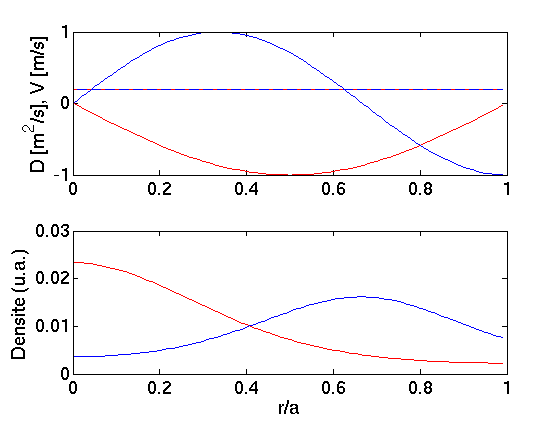
\includegraphics[width=0.70\textwidth]{Fig_Sens_piquage.png}
	\caption{Top: two cases of convection velocity radial profiles (for clarity, we have chosen identical, flat diffusion coefficient profiles indicated bi the two-colors line). Bottom: resulting density profiles in stationary states. The velocity direction has an influence on the density profile shape. When the velocity is negative (inward, red curves), the density profile is peaked. When the velocity is positive (outward, blue curve), the profile is hollow.}
	\label{fig:Sens_piquage}
\end{figure}

The same comment could be made for the temperature profile when using the heat transport equation but in general the heat sources are distributed in the plasma, which does not allow to solve the problem without a specific model.	

It is to be noticed that in the stationary case, the density profile measurement is not enough to determine separately $D$ and $V$. This determination can be done only by studying a transient state.

The difference between the study of a stationary state and that of a transient state is at the basis of heat transport experiments. Let us look again at the generic heat flux expression:

	\[
	q_e = -n_e\chi \nabla T_e
\]
Formally, the diffusivity can be deduced from the heat flux and temperature gradient measurements:
	\[
	\chi = -\frac{q_e}{n_e \nabla T_e}
\]
In practice, $\chi$ is in general a function of other gradients (which corresponds to non diagonal terms in the transport matrix, as will be seen in the next section). By isolating te term which depends only on $\nabla T_e$, we can write:
	\[
	q_e = -n_e\chi_e\nabla T_e + q_{offset} \mbox{, where } q_{offset} = \sum{M_{ij}\nabla u_j}
\]
In the case of a stationary plasma, we can deduce from the measurements:
	\[
	\chi_{stat} = -\frac{q_e}{n_e\nabla T_e} = \chi_e - \frac{q_{offset}}{n_e \nabla T_e}
\]
and in the case of a transient:
	\[
	\chi_{tr} = - \frac{\partial q_e}{n_e \partial \left( \nabla T_e\right)} = \chi_e
\]

The coefficients determined by these two methods are different, although they both represent a diffusivity. The difference between the two contains information on the dependence of diffusivity in other gradients of the plasma. The role of these other gradients must be investigated with speific experiments.
				
				
				\subsection{Transport matrix}
				\label{sub:MatriceDeTransport}

The flux expressions as functions of the associated plasma quantities suggest a matrix-like writing:
				
\[
	\Phi = M \nabla U
\]
where $\Phi$ is flux vector and $U$ is the vector of the associated plasma quantities. Let us take as an example the simple case where only the electron particle and heat fluxes are considered: 

	\[
	\Phi = \left(
								\begin{array}{c}
									q_e				\\
									\Gamma_e
								\end{array}
				 \right)
	\mbox{, }
	U =		\left(
								\begin{array}{c}
									T_e				\\
									n_e
								\end{array}
				 \right)
\]
but a more complete and detailed matrix can be built with the heat and particle fluxes for electrons, ions and the various types of impurities involved in the case under study.

The diagonal elements of this matrix are the diffusion coefficients (multiplied by density for the heat part). If for instance  electrons, ions and an impurity species are to be studied, one will have: 
	\[
	\Phi = \left(
								\begin{array}{c}
									q_e				\\
									q_i				\\
									q_Z				\\
									\Gamma_e	\\
									\Gamma_i	\\
									\Gamma_Z
								\end{array}
					\right)
		\mbox{, }
		U = \left(
								\begin{array}{c}
									T_e				\\
									T_i				\\
									T_Z				\\
									n_e				\\
									n_i				\\
									n_Z
								\end{array}
				 \right)
\]
and the transport matrix diagonal will be:
	\[
	M_{diag} = 	\left(
								\begin{array}{cccccc}
									-n_e\chi_e	&				0			&				0			&		0		&		0		&		0		\\
											0				&	-n_i\chi_i	&				0		 	& 	0 	&		0		&		0		\\
											0				&				0			&	-n_Z\chi_Z	& 	0 	&		0		&		0		\\
											0				&				0			& 			0			&	-D_e	&		0		&		0		\\
											0				&				0			&				0			&		0		&	-D_i	&		0		\\
											0				&				0			&				0			&		0		&		0		&	-D_Z
								\end{array}
							\right)
\]

We will see later that the convection velocity of a given impurity type caused by binary particle collisions depends on gradients:
	\[
		\Gamma_Z = -D_Z \left[	
													\nabla n_Z - \left(	
																					\frac{ \nabla n_i}{n_i} + ZH_Z \frac{\nabla T_i}{T_i}
																			 \right) n_Z
										\right]
\]
These dependences will be included in the transport matrix in the form of non diagonal terms.

In order to obtain simple flux expressions with only diffusion-like terms (i.e. in the form $\Phi = -D\nabla U$),we can diagonalise the transport matrix. The eigenvector basis in which it is diagonal is a linear combination of physical states. For instance, if we are interested in a situation where only the electron heat and particle fluxes must be taken into account, the basis iin which the matrix is diagonal will be made of linear combinations of $T_e$ and $n_e$. The eigen states thus do not have a clear physical meaning. To each eigenstate is associated an eigenvalue wich is the time constant characteristic of the eigenstate evolution. Conversely, each physical quantity is a linear combination of the eigenstaes. It is thus characterised by several time constants. This somewhat abbstract observation has been done also on experimental results.

Finally, there also exist terms (such as the convection velocity due to the Ware effect) which do not depend on the gradients. They are introduced on the transport matrix in a somewhat artificial way, a consequence of which is that the transport matrix is not unique.

As we have seen, the transport matrix, whose definition seems natural given the form taken by the fluxes in most theoretical models, is thus a delicate object as far as handling and interpetation are concerned. It can be useful since it allows to retrieve the characteristic time constants of a problem but it refers to quantities whose physical meaning is uncertain and abstract. 

				\subsection{Linearisation of the transport equations}
				\label{sub:LinearisationDesEquationsDeTransport}

The interest of transients for the experimental transport determination has been shown above. This is why transport experiments consist often in perturbing a stationary plasma state by a heat pulse or a particle injection. To reveal the type of transport which governs the stationary state under study, these perturbations must be small. This is the framework in which we are going to exhibit more prooperties of the generic transport model.
	
If the stationary plasma state is weakly perturbed, the evolution equations of §\ref{subsub:DefinitionDuModele} can be rewritten using the following definitions:

\begin{eqnarray}
	n 			&	=	& n_{eq} + \tilde{n}	\nonumber	\\
	T 			&	=	& T_{eq} + \tilde{T}	\nonumber	\\
	\ldots	&		&											\nonumber	\\
	\Gamma	&	=	& \tilde{\Gamma}			\nonumber	\\	
	q 			&	=	& \tilde{q}						\nonumber	\\
	\ldots	&		&											\nonumber	\\
	S_p 		&	=	& \tilde{S_p}					\nonumber	\\
	S_h 		&	= &	\tilde{S_h}					\nonumber	\\
	\ldots	&		&											\nonumber
\end{eqnarray}
where $n_{eq}$ and $T_{eq}$ are the density and temperature of the stationary state, $\tilde{n}$ and $\tilde{T}$ are the associated fluctuations, and the same notations are used for the fluxes (to retain simple expressions, sources and fluxes are assumed to be 0 for the stationary states).

Without any assumption on the flux form (e.g. the particle flux may depend on density, temperature, etc. and their gradients), the perturbed particle flux can be written as:
\begin{eqnarray}
	\tilde{\Gamma} & = & \frac{\partial \Gamma}{\partial \left( \nabla n \right)}\nabla \tilde{n} + \nonumber	\\
								&		& \frac{\partial \Gamma}{\partial \left( \nabla T \right)}\nabla \tilde{T} + 
													\ldots  + \nonumber	\\
								&		& \frac{\partial \Gamma}{\partial n}\tilde{n} + \frac{\partial \Gamma}{\partial T}\tilde{T}
													+ \ldots
\end{eqnarray}
The first line represents the diagonal term (diffusion). The second line represents the dependence of the particle fluw on the graidents other than the density gradient, i.e. the non diagonal terms of the problem. The third line represents the convective terms. The ellipsis contains the dependences on other gradients (e.g. that of another type of particles).

In the same way, the perturbed heat flux can be expressed as:
\begin{eqnarray}
	\tilde{q} & = & \frac{\partial q}{\partial \left( \nabla T \right)}\nabla \tilde{T} + \nonumber	\\
								&		& \frac{\partial q}{\partial \left( \nabla n \right)}\nabla \tilde{n} + 
													\ldots  + \nonumber	\\
								&		& \frac{\partial q}{\partial T}\tilde{T} + \frac{\partial q}{\partial n}\tilde{n}
													+ \ldots
\end{eqnarray}
Taking into account these expressions, the evolution equations expressed in amatrix form become:
\begin{eqnarray}
	\frac{\partial}{\partial t} \left( \begin{array}{cc}
																				\tilde{n}	\\		
																				\tilde{T}
																		 \end{array}
															\right)
																			& = &	-\nabla \left(
																												\begin{array}{cc}
																														\tilde{\Gamma} \\
																														\tilde{q}
																												\end{array}
																										\right)
																						+ \left(
																									\begin{array}{cc}
																											\tilde{S_p}	\\
																											\tilde{S_h}
																									\end{array}
																							\right)				\nonumber		\\
																			& = & A \nabla^2 \tilde{U} + B \nabla \tilde{U} + C\tilde{U} + \tilde{S}
\end{eqnarray}
by writing: 
\[
\tilde{U} = \left( \begin{array}{cc} 
							\tilde{n} \\ 
							\tilde{T}  
					 \end{array} 
		\right) \mbox{ et } 
\tilde{S} = \left( \begin{array}{cc}
							\tilde{S_p} \\ 
							\tilde{S_h} 
					 \end{array} 
		\right)\mbox{.}
\] 

The first term corresponds to diffusion, the second one to convection, the third is a damping term (if the C coefficients are negative). Note that $A$, $B$ and $C$ are matrices which contain the flux dependences on the plasma quantities and their gradients. Fro instance, the matrix elements of $A$ cna be easily calculated:

\[
\begin{array}{ll}
		A_{11} = \frac{\partial\Gamma}{\partial (\nabla n)}		&		A_{12} = \frac{T_{eq}}{n_{eq}} \frac{\partial\Gamma}{\partial(\nabla T)}		\\
		A_{21} = \frac{2}{3}\left( \frac{\partial\Gamma}{\partial (\nabla n)} + \frac{1}{T_{eq}}\frac{\partial q}{\partial (\nabla n)} \right)													&  A_{22} = \frac{2}{3}\left( \frac{1}{n_{eq}}\frac{\partial q}{\partial (\nabla T)} + \frac{T_{eq}}{n_{eq}}\frac{\partial\Gamma}{\partial\nabla T} \right)
\end{array}
\]

The diagonal coefficients $A_{11}$ and $A_{22}$ correspond to the heat and particle diffusion coefficients (with a $n_{eq}$ factor for the former), as already said.

We can deduce a few properties from this result. An example will be given now. Let us consider the simple case of an experiment where only one quantity is perturbed, excluding all others. The transport matrix is reduced to only one line. Let us assume in addition that we are in a purely diffusive case in one dimension. The only evolution equation is thus:

\[
	\frac{\partial u}{\partial t} = -D \frac{\partial^2 u}{\partial x^2}
\]
In the case of a sine-like periodic perturbation, the boundary conditions are:
\[
\begin{array}{ll}
		u(x=0,t) = u_0 e^{i\omega t} \\
		u(\infty, t) = 0
\end{array}
\]
the solution of this equation is:
\[
	u = u_0 e^{-x/\lambda}e^{i(\omega t - kx)}
\]
The complete resolution shows that the characteristic decay length and the phase velocity of the perturbation are:
\begin{eqnarray}
	\lambda = \sqrt{\frac{2D}{\omega}}	\nonumber	\\
	v_\phi = \sqrt{2\omega D}						\nonumber	
\end{eqnarray}

A high frequency (or fast) perturbation thus penetrates faster but shallower than a low frequency (or slow) perturbation. This property, among others, is used in the Fourier analysis method commonly used in heat transport studies.






% II. Transport collisionnel
%\chapter{Collisional transport}
\label{chap:TransportCollisionnel}


This theory was developed in the 60-70s. First it has obtained results on electron particle and energy transport, then on impurities. The object of this section is to summarise the mst important results of the theory, with a few calculations to illustrate the physics at play.



		\section{Motivations}
		\label{sec:TransportCollisionnelMotivation}

Up to now, the transport properties in tokamak plasmas have been demonstrated with a minimum number of hypotheses and very general evolution equations. Now we are going to be concerned with the first theory which has attempted to describe the nature of transport and the physical quantities which play a role in it. This theory, often called 'neoclassical theory', aims at calculating the various heat and particle fluxes due to collisions between charged particles.

first let us consider that these collisions give rise only to diffusion of particles in the plasma. an estimate of the resulting diffusion coefficient can be obtained by assuming that the (radial) displacement of a charged particle due to a collision is of the oredr of the Larmor radius. Let us denote $\nu_c$ the collision frequency of this particle. Its diffusion coefficient can be written:

\[
		\chi = \rho_L^2 \nu_c
\]

The particle lifetime in the plasma is then of the order of:
\[
\tau \simeq \frac{a^2}{\chi} = \frac{a^2}{\rho_L^2}\frac{1}{\nu_c}
\]

With reasonable values $a = 1$ m, $\rho_L = 10^{-3}$ m and $\nu_c = 250$ s$^{-1}$, we find $\tau \simeq 4\times 10^3$ s which is obviously much longer than any measured value in a tokamak. In the simplistic configuration assumed here (no force is applied ot the charged particles) the (vertical) curvature drift is responsible for a vertical electric field which causes an electric drift directed outward (away from the plasma magnetic axis). This drift drives the particles out of the plasma in less than 1 ms. This is why the tokamak magnetic configuration has been chosen: the curvature drift forces the particles to remain in the vicinity of their magnetic surface and thus reduced the electric drift effet. 

Let us now consider a situation closer to the tokamak one: cylindrical geoemtry, a magnetic field $\vec{B}$ and an elecrtric field $\vec{E}$ imposed from outside. The generalised Ohm's law can be expressed as:
\begin{equation}
	\vec{E} + \vec{v}\times\vec{B} = \eta\vec{j} + \frac{1}{en}\left( \vec{j}\times\vec{B} - \vec{\nabla}p \right)
	\label{LoidOhm}
\end{equation}
where $\eta$ is the plasma resistivite.
In addition, the pressure balance equation is:
\[
	\vec{j}\times\vec{B} = \vec{\nabla}p
\]
The vector multiplication of equation \ref{LoidOhm} by $\vec{B}$ and the use of the pressure balance equation allow to obtain:
\[
	\vec{E}\times\vec{B} - \vec{v}_{perp}B^2 = \eta\vec{\nabla}p
\]
or equivalently:
\[
		\vec{v}_{perp} = -\frac{\eta}{B^2}\vec{\nabla}p + \frac{\vec{E}\times\vec{B}}{B^2}
\]
 
The first term of the perpendicular velocity is due to collisions (as indicated by the $\nabla p$ term), the second one being the electric drift.

The particle flux associated with collisions is thus:
\[
	\vec{\Gamma}_{perp}^{coll} = nv_{perp}^{coll} = -\frac{\eta n}{B^2}\vec{\nabla} p
\]
If the temperature is uniform, we have $\vec{\nabla}p = T\vec{\nabla}n$, which gives:
\[
\vec{\Gamma}_{perp}^{coll} = -\frac{\eta \beta}{2\mu_0}\vec{\nabla}n
\]
where $\beta$ is the kinetic to magnetic pressure ratio:
\[
	\beta = \frac{nT}{B^2/2\mu_0}
\]
We cna then deduce the so-called \textit{classical} diffusion coefficient:
\[
		D_{cl} = \frac{\eta\beta}{2\mu_0}
\]



		
		\section{Collision frequency}
		\label{sub:FrequenceDeCollision}
			
			
				\subsection{Debye length}
				\label{subsub:LongueurDeDebye}


Due to the long range of the electromagnetic interaction, in principle the Coulomb interactions occur between any charged particle pair, whatever the distance between the two particles. Actually, beyond a certain distance (called \textit{Debye length}), the particles do not see each other because of a screening effect. The Debye length has the following expression:
\begin{equation}
		\lambda_D = \sqrt{\frac{\epsilon_0 kT}{n e^2}}
		\label{Debye}
\end{equation}
where $T$ and $n$ are the plasma temperature and density respectively and $e$ is the particle charge. It is assumed here thatthe plasma contains only one particle type. It is still valid if the plasma impurity content is not too high.

Each particle is sensitive to the electrostatic potential due to all the surrounding charges within a distance less than $\lambda_D$. This part of the space is referred to as the Debye sphere, volume $4/3(\pi\lambda_D^3)$, centered at the considered particle and moving with it. We will consider that the screening effect is perfect, i.e. that there are no Coulomb interactions of a particle with those outside this sphere.

The movement of each particle is influenced at every time by the potential created by its neighbours inside the Deby sphere, and these neighbours are themselves subject to the same rule. As a consequence, there are weak and fast variations of the electrostatic potential at each point of the plasma. These fluctuations are at the origin of electrostatic turbulence, qui is not taken into account in the neoclassical theory because it requires specific developments. Transport due to electrostatic turbulence is described in Chapter \ref{chap:TransportTurbulent}.


				\subsection{Landau length}
				\label{DistanceDeLandau}


Due to electrostatic repulsion, there is a lower bound for the distance between two charged particle with same sign charges. This limit is called the \textit{Landau length}. It can be easily calculated with the help of the energy conservation law in the frame of one of the particles (particle 1 in the following). The energy conservation of particle 2 writes:

\[
			E_2 = \mbox{constante, avec } E_2 = E_{p_2} + E_{c_2},
\]
$E_{p_2}$ and $E_{c_2}$ are the potential energy and kinetic energy of particle 2. At infinity, $E_{p_2} = 0$, which implies that $E_2 = E_{c_2}^\infty = kT$. Ath minimal distance $\lambda_L$, we have $E_{c_2} = 0$ and hence $E_{p_2} = kT$. Since the potential energy is due to the electrostatic potential, we have $E_{p_2} = e_1 e_2 / 4\pi\epsilon_0\lambda_L$. We can then deduce the Landau length:
\begin{equation}
		\lambda_L = \frac{e_1 e_2}{4\pi\epsilon_0 kT}.
		\label{Landau}
\end{equation}

In a tokamak plasma, the typical temperatures are around 100 eV at the edge and 10 keV in the centre. The Landau length for the plasma ions thus range from $10^{-11}$~m to $10^{-13}$~m: the fusion reactions, due to the strong interaction (range $10^{-15}$~m), occur mainly thanks to the tunnel effect.


						
				\subsection{Calculation of the collision frequency}
				\label{subsub:CalculDeLaFréquenceDeCollision}

A 'collision' between two charged particles in a plasma cannot be described as that of two billiard balls. Therre is neither impact nor contact but onyl deflection. The problem is generally treated under the name of \textit{Rutherford scattering} and the result is the deflection angle of the projectile as a function of its initial trajectory distance to the target. This distance is called the impact paramtere and will be dented $b$ in the following. In a tokamak plasma a particle is deflected more or less permanently by a multitude of interactions with its neighbours. Most of the time, these interactions occur at fairly large impact parameters and thus cause small deflections. Moreover, as a particle moves with its Debye sphere, no binary collision is complete. This is thus far from the academic Rutherford scattering case. Even the definition of a collision becomes a problem. What is the limit deflection angle (or impact parameter) above (below) which we consider a collision has occurred?

This question is answered by defining a collision by its effect. The trajectory modification corresponding to what will be called a collision is fixed arbitrarily. One of the possible criteria is that the total deflection angle resulting from a series of distant binary collisions be 90°. Another criterion is that the variation of the velocity module of a particle $\Delta v = \sum{||\delta \vec{v}||}$ be equal to $v$. Our choice for the calculation to follow concerns the velocity square. A collision will be saisd to occur when:
\[
		\Delta v^2 = \sum{(\delta v)^2} = v^2.
\]

Let us go back to the elementary case of a binary collision between a projectile (moving particle, subscript 1) and a target (unmoving particle, subscript 2). The second Newton's law allows to write the variation rate of the moving particle speed as a function of its distance $r_{12}$ to the target particle:
\[
		\frac{dv_1}{dt} = \frac{e_1 e_2}{4\pi\epsilon_0 m_1 r_{12}^2}
\]
Most of the binary interaction occur at large impact parameter. They cause alomost no deflection dunring the approach and escape phases. Their effect will be coonsidered only when particle 1 is in the vicinity of particle 2, i.e. when $r_{12} \simeq b$. This phase lasts only for approximately $\delta t \simeq b/v_1$. The speed change due to a binary collision is thus:
\[
		\delta v_1 \simeq \frac{e_1 e_2}{4\pi\epsilon_0 m_1 v_1 b}.
\]
Note that it decreases when the speed is increased. This trend will appear again in the collision frequency.

We are now going to calculate the variation of the square module of the velocity over a longer time interval  $\Delta t$. During $\Delta t$ and for an impact parameter between $b$ and $b+db$, particle 1 will be interacting with $n_2 \times 2\pi b.db.v_1.\Delta t$ particles of population 2. The speed change associated with impact parameter $b$ is thus:
\[
		\Delta (v_1^2)_b = \sum{(\delta v_1)^2} = \left( \frac{e_1 e_2}{4\pi\epsilon_0 m_1 v_1 b} \right)^2 \times 2\pi b.db\times n_2 v_1 \Delta t
\]
and, for all possible values of the impact parameter:
\begin{eqnarray}
		\Delta (v_1^2) 	&	=	&	\int_{b_{min}}^{b_{max}} \Delta (v_1^2)_b \nonumber\\
										& = &	\int_{b_{min}}^{b_{max}} \left( \frac{e_1 e_2}{4\pi\epsilon_0 m_1 v_1 b} \right)^2 \times 2\pi b.db\times n_2 v_1 \Delta t	\nonumber	\\
										& \simeq &	\frac{e_1^2 e_2^2}{\left( 4\pi\epsilon_0 \right)^2 m_1^2 v_1}.n_2\ln{\frac{b_{max}}{b_{min}}}\Delta t
\end{eqnarray}
(we have put aside a factor $2\pi$ in order to retrieve the usual expression of the collision frequency). The minimum impact parameter $b_{min}$ is that below which no collision occurs. In practice this bound can be set to the Landau length, which strictly speaking is not an impact parameter (it is the minimal distance between two particles in a front collision, i.e. $b = 0$) but is small compared to the average distance between particles ($1/n^3$).

The maximum impact parameter $b_{max}$ is that beyond which there is no interaction . It is the definition of the Debye length, hence $b_{max} = \lambda_D$. The term $\ln{\lambda_D/\lambda_L}$ is often written $\ln \Lambda$. It is called the Coulomb logarithm. Whatever the experimental situation it is always in the range 10 to 20 (more often 15 to 18).

The collision frequency definition we have chosen means that $\Delta v_1^2 = v_1^2$ when $\Delta t = 1/\nu_{12}$, $\nu_{12}$ being the collision frequency of a particle of type 1 in a population of type 2. It can be easily deduced that: 
\begin{equation}
		\nu_{12} = \frac{e_1^2 e_2^2}{\left( 4\pi\epsilon_0 \right)^2 m_1^2 v_1^3}.n_2\ln{\Lambda}
\end{equation}

Let us recall that this expression is valid in the case of a moving particle of type 1 and an unmoving population of type 2. Therefore it can be applied to calculate the collision frequency of an electron (light and thus fast) on a population of ions (heavy and thus almost at rest):
\[
		\nu_{ei} = \ln{\Lambda} \frac{e^4}{\left( 4\pi\epsilon_0 \right)^2 \sqrt{m_e} kT_e^{3/2}}.n_i
\]

It is not exactly applicable to the collision frequency of electrons onto themselves or of ions onto themselves but still it is often used with a correction factor $1/\sqrt{2}$:
\[
		\nu_{ee} = \ln{\Lambda} \frac{e^4}{\sqrt{2}\left( 4\pi\epsilon_0 \right)^2 \sqrt{m_e} kT_e^{3/2}}.n_e = \frac{1}{\sqrt{2}} \frac{n_e}{n_i}\nu_{ei}
\]
and
\[
		\nu_{ii} = \ln{\Lambda} \frac{e^4}{\sqrt{2}\left( 4\pi\epsilon_0 \right)^2 \sqrt{m_i} kT_i^{3/2}}.n_i = \sqrt{\frac{m_e}{m_i}} \left( \frac{T_e}{T_i} \right)^{3/2} \frac{n_i}{n_e}\nu_{ee}
\]

To calculate $\nu_{ie}$, let us work in the general situation i.e. without any assumption on the particle mass or speed. The momentum variation of particle 1 in the population 2 is:
\[
\frac{d\vec{p}_1}{dt} = m_1 \nu_{12} \left( \vec{v}_1 - \vec{v}_2 \right)
\]
La variation de la quantité de mouvement totale de la population 1 est donc:
\[
\frac{d\vec{P}_1}{dt} = n_1 m_1 \nu_{12} \left( \vec{V}_1 - \vec{V}_2 \right)
\]
where $\vec{V}_1$ and $\vec{V}_2$ are the average speeds of the populations. This variation corresponds to the friction force $\vec{F}_{21}$ exerted by population 2 on population 1. Following the third Newton's law (the action-reaction principle) population 1 exerts a force of same intensity and opposite direction on population 2: $\vec{F}_{12} = - \vec{F}_{21}$, which we use to find the relation between $\nu_{12}$ et $\nu_{21}$:
\[
		n_1 m_1 \nu_{12} = n_2 m_2 \nu_{21}
\]
We can deduce the collision frequency of ions onto electrons:
\[
		\nu_{ie} = \ln{\Lambda} \frac{e^4}{\sqrt{2}\left( 4\pi\epsilon_0 \right)^2 m_i^2 \left(\frac{kT_e}{2m_e} \right)^{3/2}}.n_e = \left( \frac{m_e}{m_i} \right)^2 \nu_{ee}
\]
With the assumptions $n_e = n_i$ and $T_e = T_i$, we thus have the ordering:
\[
		\nu_{ie} << \nu_{ii} << \nu_{ee} \simeq \nu_{ei}
\]

We can see that the ion thermal equilibration time is shorter than the electron-ion energy equipartition time. It could be demonstrated also that the collision frequency of impurities on ions is large enough for the two populations to be always at the same temperature.






										
		\section{Collisional regimes}
		\label{sub:RegimesCollisionnels}
				
On the basis of simple consideration on the propoerties of charged particle trajectories in tokamaks, it can be demonstrated that the diffusion coefficient takes different forms according to the range in which the collision frequency lies. This is what we are going to show now.


-------------------------------------------------

				
				\subsection{Reminder on trajectories}
				\label{subsub:RappelsTrajectoires}
						
Most of this reminder concerns trapped particle trajectories:
\begin{itemize}
		\item Trapping condition:	$\left( v_\| / v_{\bot} \right)_{\theta = 0} \leq \sqrt{2\epsilon}$
		\item Banana orbit width:	$\delta_b \simeq \frac{mv_\phi}{eB_\theta} \simeq \frac{2q}{\sqrt{\epsilon}}\rho_L$
		\item Detrapping frequency:	$\nu_{eff} = \nu_c/2\epsilon$
		\item Bounce frequency:	$\nu_b = v_\| / 2\pi q R \simeq v_{th}\sqrt{\epsilon} / 2\pi q R$
		\item Fraction of trapped particles: $f_p = \sqrt{2\epsilon}$
\end{itemize}
The inverse aspect ratio is denoted $\epsilon = r/R$ and the collision frequency $\nu_c$.

We define also the transit time of passing particles as the time necessary for them to go from the low field side midplane to the high field side midplane (or the opposite way): $\tau_\| = \pi q R / v_{th}$. To this time we associate the transit length $L_\| = \pi q R$ and the transit frequency $\nu_\| = 1/\tau_\|$.
						
						
				\subsection{Strongly collisional regime: Pfirsch-Schlüter}
				\label{RegimePfirschSchluter}
	
In this regime the mean free path of passing particles is shorter than the transit length, which writes:
\[
		\nu_c >> \frac{v_\|}{L_\|} \simeq \frac{v_{th}}{\pi qR}
\]
assuming $v_\| \simeq v_{th}$. In the random walk process already discussed, we will asume now that the elementary deviation due to a collision is of the order of the displacement due to the vertical drift during time $\tau_\|$:
\[
		\Delta = v_d \tau_\| = \frac{\rho_L}{R}v_{th}\tau_\| = \pi q \rho_L
\]
The diffusion coefficient in this case is thus:
\[
		D_{PS} = \Delta^2 \nu_c = \pi^2 q^2 \rho_L^2 \nu_c
\]
It is proportional to the collision frequency.



				\subsection{Weakly collisional regime: banana}
				\label{RegimeBanane}


We consider now a situation in which the detrapping frequency is so small that trapped particles can travel several time their orbit before being detrapped:
\[
		\nu_{eff} << \nu_b \Longleftrightarrow \nu_c << \frac{v_{th}}{\pi q R}\epsilon^{3/2}
\]
It is easily checked that in this case the collisions between passing particles are extremely rare. On the cotrary, trapped particles can have several collisions on their orbit before they are detrapped. Each collision modifies slightly their orbit and when detrapped they can leave their orbit at a radius different from that at which they were trapped. They are thus the main contributors to transport. 

The radial deviation of a particle between its trapping time and its detrapping time is of the order of the orbit width. Taking into account the fraction of trapped particles, the associated diffusion coefficient is thus:
\[
		D_B = f_p \Delta^2 \nu_{eff} = \frac{q^2 \rho_L^2}{\epsilon^{3/2}}\nu_c
\] 

	
	
				\subsection{Intermediate regime: plateau}
				\label{RegimePlateau}

\hspace{1cm} Between the two extreme regimes, only a part of the trapped particles will have many collisions before being detrapped (passing particles are still very weakly collisional). This part is of the order of $\nu_b/\nu_{eff}$. The diffusion coefficient in this regime is thus:
\[
		D_P = \frac{\nu_b}{nu_{eff}}D_B = \frac{q}{R}\rho_L^2 v_{th}
\]

The existence of three collisionality regimes is illustrated in Fig. \ref{fig:Regimes_collisionnels} for typical values of Tore Supra and ITER presented in Table \ref{tab:Regimes_collisionnels}.


\begin{figure}[htbp]
	\centering
		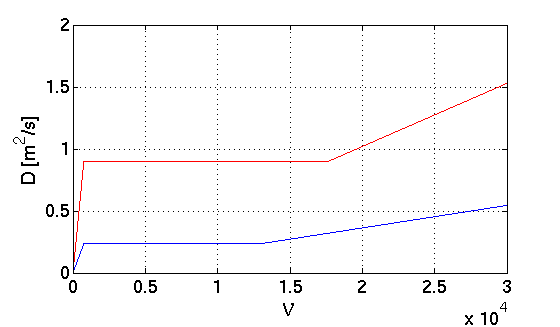
\includegraphics[width=0.70\textwidth]{Fig_Regimes_collisionnels.png}
	\caption{Dependence of the neoclassical diffusion coefficients as a function of collisionality. Electrons are always in the banana regime($\nu_e* \simeq 0,2$ in Tore Supra et 0,06 in ITER),ions are between banana regime and plateau regime, impurities are in the plateau (light impurities or very hot plasmas) or Pfirsch-Schlüter (heavy impurities or colder, thinner plasmas) regime.}
	\label{fig:Regimes_collisionnels}
\end{figure}
\begin{table}[htbp]
	\centering
		\begin{tabular}{|c|c|c|}
			\hline
			Grandeur											&		Tore Supra				&		\textit{ITER}	\\
			\hline
			B (T)													&				3,8						&		8							\\
			R	(m)													&				2,35					&		6							\\
			r (m)													&				0,35					&		0,7						\\
			q															&				2							&				2					\\
			kT (keV)											&				1							&				10				\\
			mc$^2$ (keV) =	m$_D c^2$			&	$2\times 10^6$			&	$2\times 10^6$	\\
			e	(C)													&		1,6.10$^{-19}$ 		&	1,6.10$^{-19}$	\\
			\hline
			$v_{th} = \sqrt{kT/m}$ (m/s)	&		$2.10^5$m/s				&	$6,7.10^5$ 			\\
			$\rho_L = m_D v_{th,D} /eB$ (m)	&			1,2.10$^{-3}$		&		2.10$^{-3}$		\\
			$\epsilon$										&				0,15					&			0,12				\\
			\hline
		\end{tabular}
	\caption{Parameter values used to draw the curves of Fig. \ref{fig:Regimes_collisionnels}}
	\label{tab:Regimes_collisionnels}
\end{table}


				\subsection{Collisionality}
				\label{Collisionnalite}

The numerical value of the collision frequency is not enough to know in which collisional regime a particle is, unless the physical and geometrical quantities of the plasma under study are known. For a more universal criterion, we define a normalised collsion frequency called \textit{collisionnality}:
\[
		\nu* = \frac{\pi q R}{v_{th}\epsilon^{3/2}}\nu_c
\]

The collisionality domains are bound by values $\nu* = 1$ (banana-plateau boundary) et $\nu* = \epsilon^{-3/2}$ (plateau-Pfirsch-Schlüter boundary). A typical value for deuterium in ITER is $\nu_D* \simeq 0,05$. Among the present day machines, only the largest ones can reach this collisionality range, and only for the high temperature scenarios.

On Fig. \ref{fig:nustar_D_Ni_39601} typical collisonality profiles are shown  in Tore Supra for the main ions species (deuterium) and nickel, taking into account the presence of intrinsic impurity species (carbon and helium).
\begin{figure}[htbp]
	\centering
		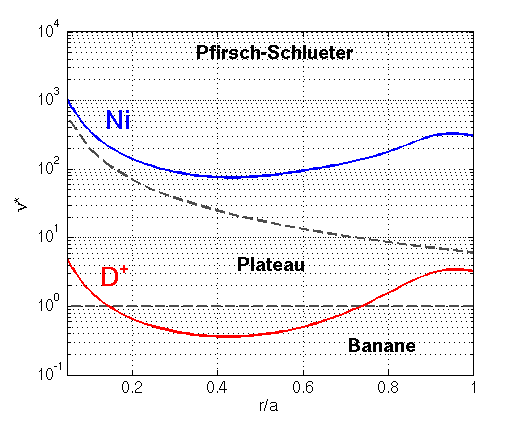
\includegraphics[width=0.70\textwidth]{Fig_nustar_D_Ni_39601.png}
	\caption{Radial profiles of collisionality for deuterium and nickel in a tore supra plasma. The dashed curves represent the boundaries of the collisionality regimes}
	\label{fig:nustar_D_Ni_39601}
\end{figure}

It can be seen that the collisional regime of a given species is not always the same in the whole plasma. In today's experiments, deuterium is often overlapping the banana and plateau regimes and the light impurities are betwqeen the plateau and the Pfirsch-Schlüter regimes. Electrons, not shown in the figure, are always deeply in the banana regime and heavy impurities in the Pfirsch-Schlüter regime.
		
		\section{Neooclassical fluxes}
		\label{sec:FluxNeoclassiques}

The heat or particle flux calculation in the frame of the neoclassical theory is complex and out of the scope of these simmple lecture notes. during the 70-80s, many authors have obtained analytical expressions, of which we are now going to give an example.

	
				\subsection{Fluid equations of motion}
				\label{sec:EquationFluideDuMouvement}


The calculation presented here relies essnetially on the resolution of the fluid equation of motion accompanied with a few assumptions and complements. This equation, which is the second moment of Vlasov equation, has the following form for a species denoted $s$:
 \begin{equation}
		n_s m_s \frac{d \vec{v}_s}{dt} = e_s n_s \left( \vec{E} + \vec{v}_s \times \vec{B} \right) - \vec{\nabla}p_s - \vec{\nabla}\stackrel{\Rightarrow}\Pi_s - \sum_{s'}n_s m_s \nu_{ss'}\left( \vec{v}_s - \vec{v}_{s'} \right)
		\label{eq:EquationFluideDuMouvement}
\end{equation}
where $n_s$, $m_s$, $e_s$, $\vec{v}_s$, $p_s$, $\stackrel{\Rightarrow}\Pi_s$  are the density, mass, charge, velocity, pressure and stress tensor associated with the particle population $s$. The sum over $s'$ concerns all the other species present in the plasma. It has the meaning of a sum oover the friction forces exerted on species $s$ by all the other species.

We will assume in the following that the plasma has a circular cross section and a large aspect ratio ($\epsilon = r/R$ is small). We will also assume that the plasma is comosed of a main ion species (denoted with subscript $D$), of an impurity species as a trace ($n_S << n_D$) and of electrons (the plasma is electrically neutral, of course). The plasma is in a stationary state: $\partial v_s/ \partial t = 0$, and the fluid velocity is much smaller than the sound speed, which allows to neglect the second term in the convective derivative ($v_s.\nabla \equiv 0$). The left hand side member of Eq. \ref{eq:EquationFluideDuMouvement} is thus 0.

The calculation will lead us to use the projections of the equation on the radial, parallel and toroidal directions. It is thus useful to give the projections of the stress tensor:

\begin{itemize}
		\item the projection in the radial direction is negligible with respect to the pressure gradient;
		\item the projection in the parallel direction is:
				\begin{equation}
							u_\|.\vec{\nabla}\stackrel{\Rightarrow}\Pi_s = \mu_s n_s m_s \nu_s \left( v_{s\theta} - k_s \frac{\nabla T_s}{e_s B_\phi} \right)
				\end{equation}
				where $\nu_s = \nu_{ss}$ et $k_s$ is a function of $n_Z$ and $e_Z$ which do not have to be specified now. finally, $\mu_s = \zeta q/\sqrt{\epsilon}$ in the banana regime, $\zeta$ being a constant;
		\item the projection in the toroidal direction is 0 because the problem is axisymmetric.
\end{itemize}

The projections of Eq. \ref{eq:EquationFluideDuMouvement} in the radial, parallel and toroidal directions are:
\begin{eqnarray}
		0	&	=	&	n_s e_s \left( E_r + v_{s\theta} B_\phi - v_{s\phi} B_\theta \right) - \nabla p_s	\label{eq:FluideDuMvt_r}\\
		0	&	=	&	n_s e_s E_\| - \mu_s n_s m_s \nu_s \left( v_{s\theta} - k_s\frac{\nabla T_s}{e_s B_\phi} \right) - \sum_{s'} n_s m_s \nu_{ss'} \left( v_{s\|} - v_{s'\|} \right)	\label{eq:FluideDuMvt_par}		\\
		0	&	=	& n_s e_s E_{ind} + e_s\Gamma_s B_\theta - \sum_{s'} n_s m_s \nu_{ss'} \left( v_{s\phi} - v_{s'\phi} \right)
		\label{eq:FluideDuMvt_tor}
\end{eqnarray}

In order to obtain the radial projections, we have neglected the radial component of the friction force because the time average of the radial component of the cyclotron velocity is 0 and the guiding centre radial velocity is small compared with its other components.

For the toroidal projection, we have assumed that $(\nabla p_s)_\phi \simeq (\nabla p_s)_\| = 0$. We have defined $\Gamma_s = n_s v_{sr}$.

In the following it will be assumed that $E_\| = E_{ind}$. Note that for a plasma with N particle species these projections give us 3N equations. Since we have 3 unknowns for each species (the three velocity components) in addition to the radial electric field, the system is under-determined. We choose here to use the radial electric field as a parameter.

Let us sum up Eq. \ref{eq:FluideDuMvt_tor} over all species. The third Newton's law requires that the friction forces cancel each other.therefore we have:
\[
		\sum_s \sum_{s'\neq s} n_s m_s \nu_{ss'} \left( v_{s\|}-v_{s'\|} \right) = 0.
\]
In addition the plasma is electrically neutral:
\[
		\sum_s e_s n_s = 0.
\]
We thus obtain the ambipolarity constraint:
\begin{equation}
		\sum_s e_s \Gamma_s = 0.
\end{equation}
This very important relation is often used in qualitative reasonings or orders of magnitude calculations.  As electroneutrality, it expresses the impossibility for the charges to be separated. However, the relations are only approximate: small deviations can happen, they are the cause of an electric field, generally a fluctuating one.

The flux of species $s$ can be expressed by subtracting Eq. \ref{eq:FluideDuMvt_par} from Eq. \ref{eq:FluideDuMvt_tor}:
\begin{equation}
		\Gamma_s = -\frac{q\mu_s}{\epsilon} \frac{n_s m_s \nu_s}{e_s B_\phi} \left( v_{s\theta} - k_s\frac{\nabla T_s}{e_s B_\phi} \right)
		\label{eq:FluxRadialGenerique}
\end{equation}
and using $B_\theta/B_\phi = r/(qR) = \epsilon/q$. It can be seen that $\Gamma_s$  is independent from $E_r$. To calculate it, we still have to calculate the poloidal velocity $v_{s\theta}$ of each species.


						
						
				\subsection{Poloidal velocity}
				\label{sec:VitessePoloidale}

						\subsubsection{Main ion}
						\label{sec:VthetaIonPrincipal}


Let us now sum up Eq. \ref{eq:FluideDuMvt_par} over all species:
\[
		\sum_s \mu_s n_s m_s \nu_s \left( v_{s\theta} - k_s \frac{\nabla T_s}{e_s B_\phi} \right) 
\]
the coefficients $\mu_e$ and $\mu_D$ being of the same order of magnitude, the elctron term, proportional to $m_e \nu_e = m_e \nu_ee$, is $(m_D/m_e)^{1/2} \simeq 60$ times smaller than the ion term proportional to $m_D \nu_D$. It can thus be neglected.
We will neglect also the impurity terms assuming trace impurities ($n_Z << n_e, n_D$). It is possible to demonstrate that this term is anyway negligible for impurities in the Pfirsch-Schlüter regime.

With these approximations the above equation provides the poloidal velocity of the main ion species:
\begin{equation}
		v_{D\theta} = k_D \frac{\nabla T_D}{e_D B_\phi}
\end{equation}
from which it is deduced that the flux of the main ion species cannot be obtained directly from Eq. \ref{eq:FluxRadialGenerique}. It will be obtained by using the ambipolarity constraint, once the poloidal velocities of the other two species are calculated.



						\subsubsection{Electrons}
						\label{sec:VthetaElectrons}

We obtain the electron poloidal velocity by subtracting Eq. \ref{eq:FluideDuMvt_r} expressed for ions and normalised to $e_D n_D$ from the same equation expressed for electrons and normalised to $e_e n_e$.

First let us write these equations:
\begin{eqnarray}
		E_r + v_{e\theta} B_\phi - v_{e\phi} B_\theta - \frac{\nabla p_e}{e_e n_e} = 0	\nonumber	\\
		E_r + v_{D\theta} B_\phi - v_{D\phi} B_\theta - \frac{\nabla p_D}{e_D n_D} = 0	\nonumber	
\end{eqnarray}
Let us subtract the second equation from the first one:
\begin{equation}
		v_{e\theta} = v_{D\theta} + \frac{B_\theta}{B_\phi}\left( v_{e\phi}-v_{D\phi} \right) - \frac{1}{B_\phi} \left( \frac{\nabla p_e}{e_e} -\frac{\nabla p_D}{e_D} \right)
		\label{eq:VitessePoloidaleElectrons_intermediaire}
\end{equation}

Assuming $v_{e\phi}-v_{D\phi} \simeq v_{e\|} - v_{D\|}$ we will obtain this term by writing Eq. \ref{eq:FluideDuMvt_par} for electrons (note that it is a form of Ohm's law) and neglecting the friction term of impurities on electrons:
\[
		v_{e\phi} - v_{D\phi} \simeq v_{e\|} - v_{D\|} = \frac{e_e E_\|}{m_e \nu_{eD}} - \mu_e \left( v_{e\theta} - k_e\frac{\nabla T_e}{e_e B_\phi} \right)
\]
or, replacing in expression \ref{eq:VitessePoloidaleElectrons_intermediaire} (assuming $n_D = n_e$) and being careful with the signs:
\begin{eqnarray}
		\left( 1 + \frac{\epsilon}{q}\mu_e \right)v_{e\theta} 	&	= &	-\frac{T_e}{e_D B_\phi} \left[ \left(1 + \frac{T_D}{T_e} \right)\frac{\nabla n_e}{n_e} + \left( 1 + \mu_e k_e\frac{\epsilon}{q} \right)\frac{\nabla T_e}{T_e} + \left( 1-k_D \right)\frac{\nabla T_D}{T_e} \right] \nonumber	\\
		&	&	- \frac{\epsilon}{q}\frac{e_D}{m_e \nu_{eD}}E_\|
\end{eqnarray}
We use the property $\mu_e \propto q/\sqrt{\epsilon}$ to neglect the terms containing $\mu_e\epsilon/q \simeq \sqrt{\epsilon}$, which is much smaller than 1, and we obtain:
\begin{equation}
		v_{e\theta} =	-\frac{T_e}{e_D B_\phi} \left[ \left(1 + \frac{T_D}{T_e} \right)\frac{\nabla n_e}{n_e} + \frac{\nabla T_e}{T_e} + \left( 1-k_D \right)\frac{\nabla T_d}{T_e} \right] - \frac{\epsilon}{q}\frac{e_D}{m_e \nu_{eD}}E_\|
		\label{eq:VthetaElectrons}
\end{equation}

In these we can see several normalised gradients $\nabla y/y$, of which the reciprocal is called a gradient length. These lengths play an essential role for neoclassical transport but we will see that their role is at least as important, if not more, for turbulent transport.


						\subsubsection{Impurities}
						\label{sec:VthetaImpuretes}


Similarly to electrons, the poloidal impurity velocity can be ontained by subtracting Eq. \ref{eq:FluideDuMvt_r} expressed for ions from the same equation expressed for the impurity:
\begin{eqnarray}
		v_{Z\theta} &	= &	v_{D\theta} + \frac{1}{B_\phi} \left( \frac{\nabla p_Z}{e_Z n_Z} - \frac{\nabla p_D}{e_D n_D} \right)			\nonumber		\\
								& = &	\frac{T_D}{e_D B_\phi} \left[ \frac{e_D}{e_Z}\frac{\nabla n_Z}{n_Z} - \frac{\nabla n_D}{n_D} + \left( k_D-1+\frac{e_D}{e_Z} \right) \frac{\nabla T_D}{T_D}\right]
								\label{eq:VthetaImpuretes}
\end{eqnarray}
We have assumed here that $T_Z = T_D$, as already discussed above.



				\subsection{Radial flux}
				\label{sec:FluxRadial}

						\subsubsection{Electrons}
						\label{sec:FluxRadialElectrons}


Injecting Eq. \ref{eq:VthetaElectrons} for the poloidal electron velocity in Eq. \ref{eq:FluxRadialGenerique} for the radial flux, we obtain the radial electron flux expression:
\begin{equation}
		\Gamma_e = - D_e\nabla n_e + V_e n_e
\end{equation}
with:
\begin{eqnarray}
		D_e	&	=	&	\zeta\frac{q^2}{\epsilon^{3/2}}\rho_e^2\nu_e \left( 1 + \frac{T_D}{T_e} \right)			\\
		V_e	&	=	&	-\zeta\frac{q^2}{\epsilon^{3/2}}\rho_e^2\nu_e \left[ \left( 1+k_e \right)\frac{\nabla T_e}{T_e} + \left( 1-k_D \right)\frac{\nabla T_D}{T_e} \right] - \zeta \sqrt{\epsilon}\frac{E_\|}{B_\theta} 
\end{eqnarray}
The calculation above, without any hypothesis on the form of the flux, evidences its nature both diffusive and convective. With a typical value of $\zeta = 2.44$ for electrons in banana regime, the diffusion coefficient $D_e$ is usually found to be of a few $10^{-3}$~m$^2$/s, which is very small (we will see that the order of magnitude for other species and for turbulent transport is much higher). It increases with $T_D/T_e$ but in most cases it is difficult to heat the ions enough to observe this effect experimentally. In ITER, $T_D$ will never be higher than $T_e$ and the effect will be modest. 

The somewhat complicated expression of the electron convection velocity $V_e$ can be approximated to its last term within a satisfactory accuracy because of the weak value of $D_e$ which multiplies the first term. The electron convection velocity is thus approximately proportional to the electrostatic field $E_\| \simeq E_{ind}$ which is induced by the magnetic flux variation in the tokamak coils. This velocity is called \textit{Ware velocity} or \textit{Ware pinch}, after the name of the physicist who discovered it by calculations and experiments. It is directed toward the magnetic axis and cancels only on plasmas where all the current is generated by non-inductive methods. This velocity is proportional to $\sqrt{\epsilon}$, which reminds us that trapped electrons are sensitive to this convective motion.


						\subsubsection{Impurities}
						\label{sec:FluxRadialImpuretes}


As for electrons, injecting Eq. \ref{eq:VthetaImpuretes} in Eq. \ref{eq:FluxRadialGenerique} , we obtain the radial impurity flux:

\begin{equation}
		\Gamma_Z = - D_Z\nabla n_Z + V_Z n_Z
\end{equation}
with:
\begin{eqnarray}
		D_Z &	=	& \frac{q}{\epsilon}\mu_Z\rho_Z^2\nu_Z			\\
		V_Z	&	=	&	-ZD_Z\left[\frac{\nabla n_D}{n_D} + \left( 1-k_D+\frac{k_Z-1}{Z} \right)\frac{\nabla T_D}{T_D}  \right]
\end{eqnarray}
and $Z = e_Z/e_D$. This expression is strictly valid only when the impurity is in the plateau regime. In the Pfirsch-Schlüter regime it takes the following form:
\begin{equation}
		\Gamma_Z = -D_Z^{PS} \left[\nabla n_Z - Z\left( \frac{\nabla n_D}{n_D} + \frac{H_Z}{K_Z}\frac{\nabla T_i}{T_i} \right)n_Z \right]
\end{equation}
with:
\begin{eqnarray}
		D_Z^{PS}	&	=	&	\nu_{ZD}q^2\rho_Z^2		\nonumber															\\
		H_Z				&	=	&	-\frac{1}{2}\times \frac{0,29 + 0,68\alpha}{0,59\alpha}	\nonumber	\\
		K_Z				&	=	&	1 - \frac{0,52\alpha}{0,59+\alpha}	\nonumber								\\
		\alpha 		&	=	&	\frac{n_Z Z^2}{n_D}
\end{eqnarray}
Actually, whatever the collisionality regime for the impurity species, the flux retains its diffusive-convective form.

These flux expressions show that the ion temperature gradient, usually negative (peaked density profile), is responsible for a convective motion toward the magnetic axis. It is thus responsible of what is called \textit{impurity accumulation}. This effect is stronger with higer impurity charges (the convective term is proportional to $Z$). In the case where the coefficient in front of $\nabla T_D/T_D$ is negative, the temperature gradient (usually negative as well) counteracts this effect: this is called \textit{temperature screening}. Due to the value of this coefficient (never more negative than -1/2) the screening effect is weaker than the accumulation effect. To prevent the peaking of the impurity density profile it is necessary to combine a rather flat ion (or electron) density profile and a fairly peaked ion temperature profile. It is in such a situation that the screening effect has been observed experimentally for the first time. The accumulation effect is often observed in good confinement regimes (H mode, ITBs) where transport is mainly collisional. In the ordinary confinement modes (ohmic, L mode), accumulation is not observed and the neoclassical predictions do not correspond to the experimental diffusion coefficients and convection velocities. These plasmas are affected by turbulence which deeply modifies the transport organisation. This is described in chapter \ref{chap:TransportTurbulent}.


		\section{Bootstrap current}
		\label{sub:CourantAutoGenere}


The results of the neoclassical theory concerning transport have rarely been in agreement with experimental results for many years.	In contrast, there is a result which was verified early: the existence of a self-generated current, often called \textit{bootstrap current}. Although it is not related to transport, it is described here because it is a part of the neoclassical theory.

		\subsection{Physical origin}
		\label{sub:OriginePhysiqueBootstrap}


Trapped particles do not contribute to the current carried by the plasma: each of these particles spends the same time travelling in one direction as in the other. However, each detrapping collision interrupts the periodical motion of a trapped particle at a random time, which breaks the symmetry.		

Let us consider two trajectories tangential to a magnetic surface, one on its inner edge and the other one on its outer edge.

\begin{figure}[htbp]
	\centering
		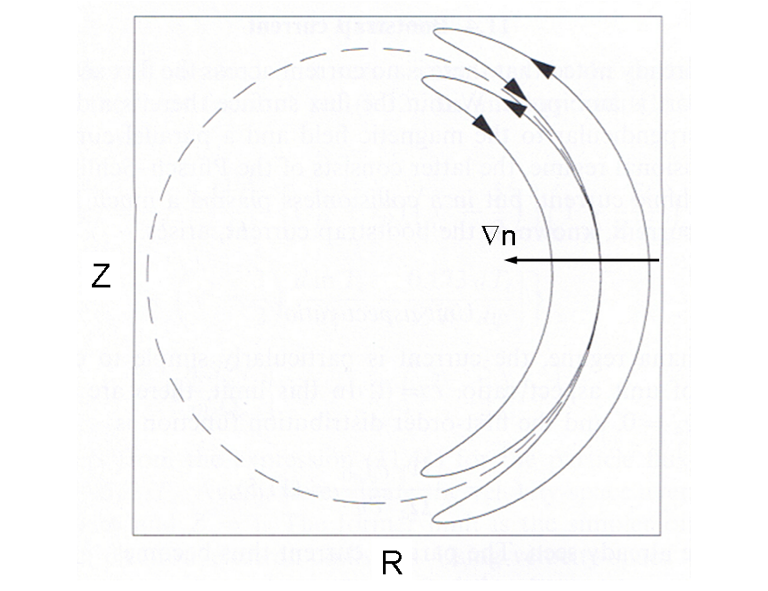
\includegraphics[width=0.50\textwidth]{Fig_bootstrap_1.png}
	\label{fig:bootstrap}
\end{figure}
If the density gradient is directed toward the magnetic axis (as usual), the particle density on the inner trajectory will be larger than that on the outer trajectory. The same comment applies of course for the number of detrapping collisions per time unit, since this number is proportional to the particle density. The net momentum transferred to passing particles due to these detrapping collisions will thus be responsible for a current.

Let us calculate the force (per unit volume) exerted by passing particles due to detrapping:
\[
		\vec{F} = \frac{d\vec{p}}{dt} \simeq \delta n.\nu_{eff}.p_\|
\]
where $\delta n$ is the density difference between the two trapped trajectories at the tangence point, $p_\|$ the particle momentum at this point and $\nu_{eff} = \nu_c/2\epsilon$ the detrapping frequency ($\nu_c$  is the collision frequency). We can express $\delta n$ in the following way:
\[
		\delta n \simeq f_p.\nabla n.\delta_b
\]
where $f_p = \sqrt{2\epsilon}$ is the fraction of trapped particles and $\delta_b = 2q\rho_L/\sqrt{\epsilon}$ is the banana orbit width. The momentum $p_\|$ given to the passing particles when a detrapping collision occurs can be assessed using the trapping condition:
\[
		p_\| = mv_\| \simeq m\sqrt{2\epsilon}v_\perp \simeq m\sqrt{2\epsilon}\sqrt{\frac{2kT}{m}}
\]
Replacing $\rho_L$ and $B_\varphi/B_\theta$ by their usual expressions, we have:
\[
		F \simeq 4\frac{m\nu_c}{eB_\theta}\sqrt{\epsilon}.kT.\nabla n
\]
During these collisions, the passing particles exert a friction force $\nu_c nmv_\|$ of same intensity and opposite sign:
\[
		\nu_c nmv_\| = 4\frac{m\nu_c}{eB_\theta}\sqrt{\epsilon}.kT.\nabla n
\]
from which we deduce the current resulting from detrapping:
\[
		j = env_\| = 4\sqrt{\epsilon} \frac{kT\nabla n}{B_\theta}
\]
This simple calculation allows to exhibit the main dependences of the bootstrap current. We are now going to calculate it in a slightly more precise way.



		\subsection{Calculation of the bootstrap current}
		\label{sub:CalculDuCourantAutoGenere}

An expression of the bootstrap current can be obtained fairly easily using the same equations as those used in the previous section.
The current carried by the plasma is by definition:
\[
		\vec{\jmath} = en \left( \vec{v}_{\varphi,i} - \vec{v}_{\varphi,e} \right)
\]
where $e$ is the proton charge, $n$ is the plasma density (we consider here a plasma of a hydrogenic species (H, D or T) without impurity: $n = n_e = n_i$), subscripts $e$ and $i$ denote electrons and ions respectively, and $v_\phi$ is a toroidal velocity.

Eq. \ref{eq:FluideDuMvt_r} allows to express $j$ as a function of the poloidal velocities:
\begin{equation}
		j = en\frac{B_\varphi}{B_\theta} \left( v_{\theta,i} - v_{\theta,e} \right) - \frac{\nabla p_i + \nabla p_e}{B_\theta}
		\label{eq:densite_courant}
\end{equation}
where $\nabla p_i$ and $\nabla p_e$ are the ion and electron pressure gradients resp. Let us remind that $\nabla p_i + \nabla p_e = \nabla p$.

Subtracting Eq. \ref{eq:FluideDuMvt_par} written for ions from the same equation written for electrons, we obtain an expression of $v_{\theta,i} - v_{\theta,e}$ as a function of the induced electric field $E_{ind}$, of the current density and of the temperature gradients:
\begin{equation}
		v_{\theta,i} - v_{\theta,e} = \left( \frac{1}{\mu_i m_i \nu_i} + \frac{1}{\mu_e m_e \nu_e} \right) e E_{ind} - \left( \frac{\nu_{ie}}{\mu_i \nu_i} + \frac{\nu_{ei}}{\mu_e \nu_e} \right) \left( v_{\|i} - v_{\|e} \right) + \frac{k_i\nabla T_i + k_e\nabla T_e}{e B_\varphi}
		\label{eq:diff_vpol}
\end{equation}

Note that with these new notations, $\nu_i$ and $\nu_e$ are the same as $\nu_{ii}$ et $\nu_{ee}$ defined in Section \ref{subsub:CalculDeLaFréquenceDeCollision}. We thus have:
\begin{eqnarray*}
		\frac{1}{m_i \nu_i} & \simeq & \sqrt{\frac{m_e}{m_i}} \frac{1}{m_e\nu_e}		\\
		\frac{\nu_{ei}}{\nu_e}	&	\simeq	&	1					\\
		\frac{\nu_{ie}}{\nu_i} &	<<	&	1
\end{eqnarray*}
In addition $\mu_e \simeq \mu_i$. this allows us to simplify Eq. \ref{eq:diff_vpol}~:
\[
		v_{\theta,i} - v_{\theta,e} = \frac{e}{\mu_e m_e \nu_e}E_{ind} - \frac{\nu_{ei}}{\mu_e \nu_e} \left( v_{\|i} - v_{\|e} \right) + \frac{k_i\nabla T_i + k_e \nabla T_e}{e B_\varphi},
\]
and replacing in Eq. \ref{eq:densite_courant}~:
\[
		j = \frac{n e^2}{m_e\nu_e \left( 1 + \mu_e\frac{B_\varphi}{B_\theta} \right)} E_{ind} - \frac{1}{1 + \frac{B_\varphi}{\mu_e B_\theta}} \frac{\nabla p - n\left( k_i\nabla T_i + k_e\nabla T_e \right)}{B_\theta}
\]

We recall that $B_\varphi / B_\theta = q / \epsilon$ et $\mu_e B_\theta / B_\varphi = C\sqrt{\epsilon} \ll 1$ (in banana regime), which we use to get a simplified expression of the current density:
\[
		j \simeq \frac{ne^2}{m_e \nu_e}E_{ind} - C\sqrt{\epsilon} \frac{\nabla p - n\left( k_i\nabla T_i + k_e\nabla T_e \right)}{B_\theta}
\]

It can be seen that the first term, proportional to the induced electric field, is the current imposed by the magnetic flux variation in the tokamak coils. The second term is present even without the inductive phenomenon. It exists as soon as there is a pressure gradient in the plasma. It is the self generated current or \textit{bootstrap current}. The factor $\sqrt{\epsilon}$ reminds us that it is due to trapped particles. 


%		\section{Vérifications expérimentales}
%		\label{sec:VerificationsExperimentales}
		
%				\subsection{Courant auto-généré}
				
%				\subsection{Ecrantage de température}
				
%				\subsection{Echecs de la théorie néoclassique}

		\section{Summary of Chapter \ref{chap:TransportCollisionnel}}
		\label{sec:ConclusionNeoclassique}
		
The evaluation of the collision frequency for charged particles of different species and the effect of collisions on the various type of trajectories (passing, trapped) allow to identify three transport regimes: from the weakly collisional to the highly collisional, the banana, plateau and Pfirsch-Schlüter regimes. Electrons are always in the banana regime, light ions are in variable situations depending on the plasma charateristics, and heavy impurities are in the Pfirsch-Schlüter regime. In a more accurate treatment of the problem (which is out of the scope of these notes), all types of trajectories contribute to transport and the total flux of a given species $s$ is of the form:
\[
		\Gamma_s = \Gamma_{cl} + \Gamma_{BP} + \Gamma_{PS}
\]
where $\Gamma_{cl}$ is the classical flux, $\Gamma_{BP}$ is the flux due to collisions involving trapped particles, dominant in the banana and plateau regimes, and $\Gamma_{PS}$ is the flux due to collisions involving  passing particles, dominant in the Pfirsch-Schlüter regime.

We have shown in a particular case that the charged particle flux, whatever the species, is of the diffusive-convective form, which justifies \textit{a posteriori} the assumption done in Chapter \ref{chap:Introduction} for the generic model. The electron convection is directed inward and proportional to the induced electric field. For impurities, we have evidenced the accumulation effect due to the ion density gradient and the temperature screening effect due to the ion temperature gradient. 

In this chapter we have ignored the existence of electromagnetic fluctuations due for instance to the small, short-lived, real charge distribution deviations from the Boltzmann distribution. The effect of these fluctutions is discussed in the next chapter. 



% III. Transport turbulent
%\chapter{Turbulent transport}
\label{chap:TransportTurbulent}

The charge density fluctuations around Boltzmann distribution are inherent to plasmas. They are on a scale shorter than the Debye length since a charged particle is sensitive only to other particles within its Debye sphere. Here it will be shown that charge density perturbations can occur on a larger scale. We will take as an example the drift wave, a typical instability in the confined plasma, but we could also consider the interchange instability. These perturbations contribute to plasma transport, which will be discussed with the help of the electric drift around the electrostatic potential extrema.

There are several possible frameworks to study the effect of turbulence on transport. The gyrofluid theory can be developed by solving the equations formed as the first moments of Vlasov's equation (averaged over the cyclotron motion) to which is added a closure relation. It is also possible to develop the gyrokinetic theory, which consists in looking for the distribution function response to a perturbation (again with an average over the cyclotron motion). For either of these two models, the theoretician can choose to study the linear plasma response to a weak perturbation - it is the quasilinear approach. It is also possible to include the interactions of the various quantities with each other - this is the nonlinear approach. A number of ingredients can be added to the model, such as the finite Larmor radius effects, various kinds of collision operators... The nonlinear gyrokinetic approach has two versions: the so-called 'local', which calculates only the deviation to the equilibrium distribution function and the so-called 'full-f' which consists in calculating the complete distribution function. The choice of the framework depends on the specific problem to be studied, on the desired accuracy and on the available computation time.

These various models will not be described in detail here but we will use one or the other depending on the specific point discussed.



		\section{Effect of fluctuations on a test particule}
		\label{sec:FluctuationsParticuleTest}
		
				\subsection{Fluctuations of the magnetic field}
				\label{FluctuationsDuChampMagnetique}

Let us make the approximation of a particle submitted to turbulence in a plasma tokamak witouht having any influence on it, as is the case when trace impuities are injected into a plasma for a transport study.

If the magnetic field $\vec{B}$  fluctuates around an average field $\vec{B}_{eq}$:
\[
		\vec{B} = \vec{B}_{eq} + \tilde{\vec{B}},
\]

The direction of the particle guiding centre, which is always aligned with the total field, will be submitted to small deviations. For instance, in the radial direction (which is still the one we are interested in), the fluctuating part of the particle velocity is given by:
\[
		\tilde{v}_r = \frac{\tilde{B}_r}{B_{eq}}v_\|
\]
The resulting radial displacement, of which the scale is denoted $\Delta$:
\[
		\Delta^2 \simeq \left< |\tilde{v}_r|^2\!\right>\tau_{c\|} = \left< \left| \frac{\tilde{B}_r}{B_{eq}} \right|^2\right> \lambda_{c\|}^2
\]
Here $\tau_{c\|}$, which is called the correlation time, is the time during which the particle is submitted to the fluctuation and $\lambda_{c\|}$, called the correlation length, is the corresponding distance in the parallel direction. If the particle is fast or if the fluctuation lifetime is long, $\lambda_{c\|}$ is the characteristic length of a $B$ fluctuation in the radial direction. On the contrary if the particle is slow or if the fluctuation lifetime is short, $\lambda_{c\|}$  is the distance travelled by the particle in the parallel direction during time $\tau_{c\|}$. In both cases, we have $\lambda_{c\|} = v_\|\tau_{c\|}$. 

An order of magnitude of the diffusion coefficient can be obtained by writing:
\[
		D_M \simeq \frac{\Delta^2}{\tau_{c\|}} = \left< \left| \frac{\tilde{B}_r}{B_{eq}} \right|^2\right> \lambda_{c\|} v_\|
\] 
This expression shows that diffusion due to the magnetic field fluctuations increases with velocity. It is thus stronger for electrons than for ions. Assuming that $\lambda_{c\|}$ is of the same order as the transit length and that the parallel velocity is equal to the thermal velocity, we have:
\[
		D_M \simeq \pi q R v_{th,e} \left< \left| \frac{\tilde{B}_r}{B_{eq}} \right|^2\right>
\]
and, with reasonable values of $q$, $R$ and $T_e$:
\[
		D_M \simeq 10^8 \left< \left| \frac{\tilde{B}_r}{B_{eq}} \right|^2\right>		\mbox{(en m$^2$/s)},
\]
which gives 1 m$^2$/s for magnetic field fluctuations of 10$^{-2}$\%.
		
		
				
				\subsection{Fluctuations of the electrostatic field}
				\label{FluctuationsDuChampElectrostatique}
		
		
Let us assume now that the fluctuations are of an electrostatic nature. The electrostatic potential will be denoted $\phi = \tilde{\phi}$ assuming that the equilibrium potential is 0 (which is true for scales longer than the Debye length.) The test particle drifts around the potential extrema because of the electric drfit:
\[
		\tilde{\vec{v}}_E = \frac{\tilde{\vec{E}} \times \vec{B}}{B^2}
\]
of which the radial projection is:
\[
		\tilde{v}_{Er} = \frac{\tilde{E}_{\theta}}{B}
\]
The radial distance travelled by the particle during the parallel correlation time is of the order of $\Delta$:
\[
		\Delta^2 = \left< |\tilde{v}_{Er}|^2\right>\tau_{c\|}^2
\]
From this we can deduce an order of magnitude of the coefficient diffusion associated with electrostatic turbulence:
\[
		D_{ES} \simeq \frac{\Delta^2}{\tau_{c\|}} = \left< \left| \frac{\tilde{E}_\theta}{B} \right|^2 \right> \lambda_{c\|}/v_\|
\]
In this case diffusion is stronger for slow particles, i.e. ions.

By definition we have $\tilde{E} = -\nabla \tilde{\phi}$ and assuming that the turbulence scale in the poloidal direction is characterised by $1/k_\theta$ we get that $\tilde{E}_\theta \simeq k_\theta \tilde{\phi}$. In addition, we can express the magnetic field as a function of the thermal velocity and the ion Larmor radius:
\[
		\frac{1}{B} = \frac{e\rho_i}{mv_{th,i}}
\] 
The diffusion coefficient associated with electrostatic turbulence can thus be expressed in the following way:
\[
		D_{ES} \simeq \pi q R v_{th,i}(k_\theta \rho_i)^2 \left< \left| \frac{e \tilde{\phi}}{T} \right|^2 \right>
\]
or, with reasonable values of the plasma quantities:
\[
		D_{ES} \simeq 10^4 \left< \left| \frac{e \tilde{\phi}}{T} \right|^2 \right>		\mbox{(en m$^2$/s)}.
\]
This ives a diffusion coefficient of 1 m$^2$/s for electrostatic potential fluctuations of 1\%. 

For a comparable diffusion coefficient, the relative level of electrostatic fluctuations must be much higher than that of magnetic fluctuations (two orders of magnitude). However anomalous transport (i.e. the difference between observed transport and the neoclassical predictions) is usually explained by the former, on the one hand because magnetic fluctuations even of a low level are hard to justify and on the other hand because the elctrostatic fluctuation level measured in tokamaks is of the order of 1\% in the centre and more than 10\% (even 100\%) at the edge. In the following, only the electrostatic potential fluctuations will be discussed.

		\section{Diffusion Quasi-linear electrostatic turbulent diffusion}
		\label{sec:DiffusionQuasiLineaire}
		
		
In Section \ref{sec:FluctuationsParticuleTest}, a relation was obtained between the turbulent diffusion coefficient and the plasma characteristics for a test particle. We are now going to look for the global plasma response assuming that the plasma responds linearly to an electrostatic potential perturbation.This situation corresponds to a 'weak' perturbation of which the average is 0 over a time long compared with the perturbation evolution time (generally called the turbulence correlation time).

As in all that has been discussed above, only the flux radial component will be considered (the other components are generally 0).We do not know its expression but the drift velocity dcalculations allow us to write the component perpendicular to the magnetic field (which contains the radial component):
\[
		\vec{\Gamma}_\perp = n \left( \vec{v}_E + \vec{v}_{dia} + \vec{v}_{pol} \right)
\]

The radial flux is the radial component of the perpendicular flux: $\Gamma_r = (\Gamma_\perp)_r$. The radial turbulent flux is the time average of this instantaneous radial flux over a time long compared with the turbulence correlation time $\tau_c$:
\[
		\vec{\Gamma}_{r,turb} = \left< \vec{\Gamma}_r \right> = \left< n \vec{v}_r \right>
\]
where $\left<...\right>$ represents the time average. these quantities are of course averages over a flux surface, i.e. over angles $\theta$ and $\varphi$.

The polarisation velocity $\vec{v}_{pol}$ is in the perpendicular direction, and its intensity is of the order of $\rho_L / L_c$ where $\rho_L$  is the Larmor radius and $L_c$ is the turbulence correlation length. The velocity $v_{pol}$ is thus significant only when $L_c$ is small, which corresponds to a situation of small scale turbulence which contributes little to transport. The effect of $v_{pol}$ will thus be neglected. We are left with:

\[
		\vec{\Gamma}_{r,turb} = \left< n \vec{v}_{Er} \right> + \left< n \vec{v}_{dia,r} \right>
\]
By taking the known expression of the diamagnetic drift velocity, we obtain:
\begin{eqnarray*}
		\left< n \vec{v}_{dia,r} \right>	&	=	&	\left< \frac{\left(\vec{B} \times \vec{\nabla}p \right)_r}{eB^2} \right>			\\
																			&	=	&	\frac{ \left( \vec{B} \times \left< \vec{\nabla}p \right> \right)_r }{eB^2}		\\
																			&	=	&	\left< \frac{\left(\vec{B} \times \vec{\nabla}p_{eq} \right)_r}{eB^2} \right>
\end{eqnarray*}
since the time average of the fluctuating pressure gradient is 0: $\left< \nabla \tilde{p} \right> = 0$. As the equilibrium pressure gradient is in the radial diractione, the diamagnetic drift velocity contribution to the turbulent flux is 0. Only the electric drift velocity contribution remains:
\[
		\vec{\Gamma}_{r,turb} = \left< n \vec{v}_{Er} \right>
\]

We are now going to use the quasilinearity assumption: we assume that the plasma quantities respond to a weak fluctuating perturbation by a weak fluctuating perturbation:
\begin{eqnarray*}
		n	&	=	&	n_{eq} + \tilde{n}		\\
		\vec{v}	&	=	&	\vec{v}_{eq} + \tilde{\vec{v}}		\\
		p	&	=	&	p_{eq} + \tilde{p},		\\
		\ldots	&	&
\end{eqnarray*}
We can re-write the total average flux:
\begin{eqnarray*}
		\vec{\Gamma}_r	&	=	&	\left< n_{eq} \vec{v}_{Er,eq} \right> + \left< \tilde{n} \tilde{\vec{v}}_{Er} \right>	\\
											&	=	&	n_{eq} \vec{v}_{Er,eq} + \left< \tilde{n} \tilde{\vec{v}}_{Er} \right>		\\
											&	=	&	\vec{\Gamma}_{r,eq} + \vec{\Gamma}_{r,turb}
\end{eqnarray*}
The dirst term is the equilibrium flux (i.e. over a time scale longer than the fluctuation time scale) and the second term is the radial flux associated with turbulence.

Before giving this flux expression, we are going to use the continuity equation to obtain the density response to this turbulent flux:
\[ 
		\frac{\partial n}{\partial t} + \vec{\nabla}.\vec{\Gamma}_r = 0
\]
Using the linearity assumption, we get:
\begin{eqnarray*}
		\frac{\partial n_{eq}}{\partial t} + \vec{\nabla}.\vec{\Gamma}_{r,eq} & = & 0		\\
		\frac{\partial \tilde{n}}{\partial t} + \vec{\nabla}.\vec{\Gamma}_{r,turb} & = & 0
\end{eqnarray*}
and thus:
\[
		\frac{\partial \tilde{n}}{\partial t} + \left< \tilde{\vec{v}}_{Er}. \vec{\nabla} \tilde{n} \right> + \left< \tilde{n} \vec{\nabla}. \tilde{\vec{v}}_{Er} \right> = 0
\]

\begin{itemize}
\item In the case of a homogeneous $B$ field, we have:
\[
		\vec{\nabla}\vec{v}_E = \vec{\nabla}. \left( \frac{\vec{B}\times\vec{\nabla}\phi}{B^2} \right) = - \vec{\nabla}. \left( \vec{\nabla} \times \left( \frac{\phi \vec{B}}{B^2} \right) \right) = 0
\]
\item In the case of an inhomogeneous $B$ field, we have:
\[
		\vec{v}_E = - \vec{\nabla} \times \left( \frac{\phi \vec{B}}{B^2} \right) + \phi \frac{\vec{\nabla}\times \vec{B}}{B^2}
\]
and thus
\[
		\vec{\nabla}. \vec{v}_E = \vec{\nabla}. \left( \phi \frac{\vec{\nabla} \times \vec{B}}{B^2} \right) = \vec{\nabla} \phi . \frac{\vec{\nabla} \times \vec{B}}{B^2}
\]
In the frame moving with speed $\vec{v}_{E,eq}$, both factors of the right hand side member are small. Indeed,  $\nabla \phi = \nabla \tilde{\phi}$ is small and $\vec{\nabla} \times \vec{B}/B$ is of the order of $1/R$. We tus neglect $\vec{\nabla}. \vec{v}_E$.
\end{itemize}
The continuity equation has thus two terms left:
\[
		\frac{\partial \tilde{n}}{\partial t} + \left< \tilde{\vec{v}}_E . \vec{\nabla}\tilde{n} \right> = 0
\]

Any perturbation can be written in the form of a Fourier series:

\begin{eqnarray*}
		\phi & = & \sum_{m,n,\omega} \phi_{m,n,\omega}(r) e^{i(m\theta + n\varphi-\omega t)}		\\
		n   & = & \sum_{m,n,\omega}    n_{m,n,\omega}(r) e^{i(m\theta + n\varphi-\omega t)}		\\
\end{eqnarray*}
which can also be written:
\begin{eqnarray*}
		\phi & = & \sum_{\vec{k},\omega} \phi_{\vec{k},\omega}(r) e^{i(\vec{k}\vec{x}-\omega t)}		\\
		n   & = & \sum_{\vec{k},\omega}    n_{\vec{k},\omega}(r) e^{i(\vec{k}\vec{x}-\omega t)}		\\
\end{eqnarray*}
with $k_\theta = m/r$ (we will not have to deal with the toroidal dimension in this calculation).

Since $\tilde{\phi}$ and $\tilde{n}$ are physical quantities (and thus real), the Fourier coefficients must verify the relation:
\begin{eqnarray*}
		\phi_{-\vec{k},-\omega} & = & \phi_{\vec{k},\omega}^*		\\
		n_{-\vec{k},-\omega} & = & n_{\vec{k},\omega}^*
\end{eqnarray*}

If $B$ is homogeneous, the fluctuating electric drift velocity becomes:
\begin{eqnarray*}
		\tilde{v}_{Er} & = & \left( \frac{\vec{B} \times \vec{\nabla}\tilde{\phi}}{B^2} \right)_r	\\
									 & = & -\frac{1}{B^2}. B.\left( \nabla \tilde{\phi} \right)_\theta = - \frac{1}{rB}\frac{\partial\tilde{\phi}}{\partial\theta},
\end{eqnarray*}
or, using the Fourier development of $\phi$:
\[
		\tilde{v}_{Er} = \sum_{\vec{k},\omega} \left( -\frac{ik_\theta}{B} \right) \phi_{\vec{k},\omega} e^{i(\vec{k}\vec{x}-\omega t)}
\]
The turbulent flux expression thus becomes:
\begin{equation}
		\vec{\Gamma}_{r,turb} = \left< \tilde{n} \tilde{v}_{Er} \right> = \sum_{\vec{k},\omega} \left( -\frac{ik_\theta}{B} \right) n_{-\vec{k},-\omega} \phi_{\vec{k},\omega},
	\label{eq:flux_turb_prov}
\end{equation}
the time average of the other terms being 0. 

The continuity equation will provide a relation between the Density Fourier coefficients and the potential ones. Without time average, it has the following form:
\[
		\frac{\partial \tilde{n}}{\partial t} + \tilde{\vec{v}}_{Er}.\vec{\nabla}n_{eq} = 0.
\]

We have neglected the term $\tilde{\vec{v}}_{E,eq}.\vec{\nabla}\tilde{n}$, which is of second order, and we have chosen the frame moving at speed $\vec{v}_{E,eq}$, so that $\vec{v}_{E,eq}.\vec{\nabla}\tilde{n} = 0$. In the Fourier space, the equation becomes:
\[
		-i\omega n_{\vec{k},\omega} = -\frac{ik_\theta}{B} \phi_{\vec{k},\omega}.\nabla n_{eq},
\]
or:
\[
		n_{\vec{k},\omega} = \frac{k_\theta}{\omega B} \phi_{\vec{k},\omega}.\nabla n_{eq}
\]
which we replace in Eq. \ref{eq:flux_turb_prov}:
\[
		\Gamma_{r,turb} = - \sum_{\vec{k},\omega} \frac{i}{\omega} \left| \frac{k_\theta}{B}\phi_{\vec{k},\omega} \right|^2 \nabla n_{eq}
\]

It is possible to show that the divergence at $\omega = 0$ comes from the fact that we have neglected the second order term $\tilde{\vec{v}}_{E,eq}.\vec{\nabla}\tilde{n}$. If it is taken into account, instead of a divergence we have a resonance of which the width is often denoted $\Delta\omega_k$. The flux expression takes the new form:
\[
		\Gamma_{r,turb} = - \sum_{\vec{k},\omega} \frac{i\omega + \Delta\omega_k}{\omega^2+\Delta\omega_k^2} \left| \frac{k_\theta}{B}\phi_{\vec{k},\omega} \right|^2 \nabla n_{eq}
\]
This expression has the form of Fick's law with a diffusion coefficient:
\[
		D_{turb} = \sum_{\vec{k},\omega} \frac{i\omega + \Delta\omega_k}{\omega^2+\Delta\omega_k^2} \left| \frac{k_\theta}{B}\phi_{\vec{k},\omega} \right|^2
\]

The proportionality between $D_{turb}$ and $\left| \phi_{\vec{k},\omega} \right|^2$ indicates that diffusion is larger for modes with a large amplitude. The quasilinear framework does not provide quantitative results on the transport coefficients. Indeed it does not allow to calculate the electrostatic potential fluctuations ( which are necessary to know the Fourier coefficients $\phi_{\vec{k},\omega}$ and the $k_\theta$ spectrum of turbulence) in physical units. Only the nonlinear theory allows a complete calculation of the flux and the associated transport coefficients.



		\section{Phase and transport}
		\label{sec:DephasageEtTransport}
		
				\subsection{General case}
				\label{sub:DephasageCasGeneral}
				
We have seen in the previous section that the turbuent particle flux can be written:
\[
		\Gamma_{r,turb} = \left< \tilde{n}\tilde{v}_{Er} \right>_{t,\theta,\phi}
\]
where $\tilde{v}_{Er}$ is the radial component of the electric drift velocity and where the flux surface average is apparent. The electric drift velocity has the form $\tilde{v}_E = \tilde{E}_\theta/B$. As a result we have $\Gamma_{r,turb} = 0$ if $\tilde{n}$ and $\tilde{E}$ (or equivalently $\tilde{\phi}$) are in phase. To be more accurate, let us write the perturbed electrostatic potential and the density response as Fourier series:
\begin{eqnarray*}
		\tilde{\phi}  &  =  &  \sum_m \hat{\phi}_m e^{i\left( m\theta + \varphi_m^\phi \right)}		\\
		\tilde{n   }  &  =  &  \sum_m \hat{n}_m e^{i\left( m\theta + \varphi_m^n \right)}	
\end{eqnarray*}
(the toroidal dependence does not appear for the sake of simplicity, but it can be calculated in the same way), where the coefficients $\hat{\phi}_m$ et $\hat{n}_m$ are real and:
\begin{eqnarray*}
		\hat{n}_m     &  =  &  \hat{n}_{-m}			\\
		\hat{\phi}_m     &  =  &  \hat{\phi}_{-m}			\\
		\hat{\varphi}_m  &  =  &  - \hat{\varphi}_{-m}
\end{eqnarray*}
to ensure that $\tilde{\phi}$ and $\tilde{n}$ are real. The turbulent flux becomes:
\begin{eqnarray*}
		\Gamma_{r,turb}  &  =  &  \sum_m i \left( \frac{m}{rB} \right) \hat{n}_m \hat{\phi}_{-m} e^{i \left( \varphi_m^n + \varphi_{-m}^\phi \right)}		\\
										 &  =  &  \sum_m \left( \frac{im}{rB} \right) \hat{n}_m \hat{\phi}_m e^{i \left( \varphi_m^n - \varphi_m^\phi \right)}		\\
										 &  =  &  \sum_{m>0} \left( \frac{2im}{rB} \right)\hat{n}_m \hat{\phi}_m \sin \left( \varphi_m^n - \varphi_m^\phi \right)
\end{eqnarray*}
The resulting turbulent flux is finite if and only if $\varphi_m^n - \varphi_m^\phi \neq 0$, which means if at least one of the Fourier contibutions is out of phase. As a consequence, the assumption of an adiabatic electron response  ($\tilde{n}/n_{eq} = e\tilde{\phi}/T_e$) does not produce any radial turbulent flux.


				\subsection{Drift wave}
				\label{OndeDeDerive}
				
				
\begin{figure}[htbp]
	\centering
		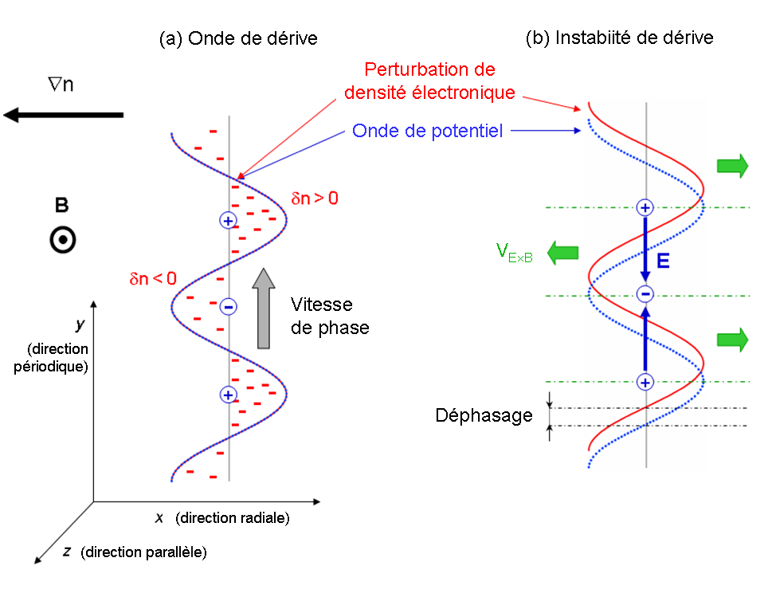
\includegraphics[width=0.70\textwidth]{Fig_onde_de_derive.png}
	\caption{Schematic representation (a) of a drift wave propagating in the poloidal direction, (b) of a drift instability driving transport).}
	\label{fig:onde_de_derive}
\end{figure}

The drift wave allows to give an example of a situation where the density response is ou of hpase with respect to the fluctuating potential excitation. Let us consider at a given time a periodical perturbation of the electrostaticpotential in the poloidal direction (denoted $y$ on the figure): $\tilde{\phi} \propto \exp{i \left( k_y y - \omega t \right)}$. If the perturbation frequency is not too large, the electron distribution adapts instantaneously to the potntial and the electron density fluctuation is in phase with that of the potential. This is called the electron adiabaticity hypothesis. The result is shown in Fig. \ref{fig:onde_de_derive}.a: over-density zones around the potential maxima alternate with under-density zones around the potential minima.
				
Let us look now at the electric drift velocities of the various zones in this simplemodel. By definition, the electric field $E_y$ is directed from the potential maxima to the potential minima, hence from the overdensity zones to the under-density zones. Taking into account the direction of $\vec{B}$ as indicated on the figure, we see that the upper (on the figure) half of an over-density zone is submitted to an outward drift, whereas the lower half is pushed inward. In the same way, the upper half of an under-density zone is pushed inward whereas the lower half is pushed outward. The global effect is the perturbation propagation in the poloidaldirection ($y$ on the figure), without amplification or damping. There is no transport in this case, which is in agreement with the result of the previous paragraph.

In the case where the density response is out of phase with the potential fluctuation (Fig. \ref{fig:onde_de_derive}.b), the symmetry between the zones pushed inward and outward is broken. The global effect is indeed that of electron trnasport. Depending on the sign of the phase sift, the phenomenon is stabilising (if the over-density zones are pushed inward and the under-density zones are pushed outward) or destabilising (in the opposite case).

\textit{Exercise: is the situation shown in Fig. \ref{fig:onde_de_derive}.b stabilising or destabilising?}

A poloidally periodic perturbation of the potential can thus be ineffective for transport (if density and potential are in phase), damped or responsible for a macroscopic transport. This third situation is the object of turbulent transport modelling.

Phase shifts between potential and density can be due to resistivity, which invalidates the electron adiabaticity hypothesis, or to resonances between wavec and particles.

		
		\section{A few propoerties of the quasilinear theory}
		\label{sec:QuelquesProprietesDeLaTheorieQuasiLineaire}
		
				\subsection{Resonance and Landau damping}
				\label{sub:ResonanceEtAmortissementDeLandau}
				
				
In the previous discussion we have used the fluid model. Now we are going to give a gyrokinetic description of the plasma. it is now described by the guiding centre distribution function, generaly denoted $f$, in the phase space. To make the developments  simpler, we will use a two dimension phase space: one for position ($r$) and one for velocitiy ($V$). With the appropriate normalisations, Vlasov's and Poisson's equations take the following forms:
\begin{eqnarray*}
		\partial_\tau f + V \partial_x f + \partial_x \phi \partial_V f = 0		\\
		\partial_x^2 \phi = \int_{-\infty}^{+\infty} f dV - 1
\end{eqnarray*}
où $\partial_a = \partial/\partial a$ et où les normalisations adoptées sont les suivantes:
\begin{eqnarray*}
		x     &  =  &  \frac{r}{\lambda_D} = \sqrt{\frac{n_e e^2}{\epsilon_0 k_B T}}r		\\
		\tau  &  =  &  \omega_{pe} t = \frac{v_{th,e}}{\lambda_D} t											\\
		V			&  =  &  \frac{v}{v_{th,e}}			\\
		\phi  &  =  &  \frac{e\Phi}{T_e}
\end{eqnarray*}
where $\Phi$ is the electrostatic potential in physical units. In addition, $f$ is normalised to $v_{th,e}/n_e$ (instead of 1).

At equilibrium (i.e. without fluctuating potential):
\[
		\partial_\tau f_{eq} = 0 \mbox{\hspace{1cm} et  \hspace{1cm}}  \phi = 0.
\]
Vlasov's equation thus becomes $\partial_x f_{eq} = 0$: $f_{eq}$ is a function only of $v$. Poisson's equation gives:
\[
		\int_{-\infty}^{+\infty} f_{eq} dv = 1
\]
The distribution function is now perturbed (weakly):
\[
		f(x,V,\tau) = f_{eq}(V) + \tilde{f} (x,V,\tau)		\mbox{\hspace{1cm} et  \hspace{1cm}}		\left< \tilde{f} \right>_{t,r} = 0
\]
Let us write Vlasov's equation again:
\[
		\partial_\tau f_{eq} + \partial_\tau \tilde{f} + V \partial_x f_{eq} + V \partial_x \tilde{f} + \partial_x\phi \partial_V f_{eq} + \partial_x\phi \partial_V \tilde{f} = 0
\]
The first and third terms are 0 for obvious reasons. The last term is of the second order and thus negligible. We are thus left with:
\[
		\partial_\tau \tilde{f} + V \partial_x \tilde{f} + \partial_x\phi \partial_V f_{eq} = 0
\]
Poisson's equation gives also some information:
\begin{eqnarray*}
		\partial_x^2\phi  &  =  &  \int_{-\infty}^{+\infty} f_{eq} dV  + \int_{-\infty}^{+\infty} \tilde{f} dV -1 \\
											&  =  &  \int_{-\infty}^{+\infty} \tilde{f} dV
\end{eqnarray*}

The plane wave functions are solutions of these equations. We are thus going to look for solutions which are linear combinations of plane waves:
\begin{eqnarray*}
		\tilde{\phi}		&		=		& \sum_{k,\omega} \hat{\phi}_{k,\omega} e^{i \left( kx - \omega \tau \right)}	\\
		\tilde{f}		&		=		& \sum_{k,\omega} \hat{f}_{k,\omega} e^{i \left( kx - \omega \tau \right)}
\end{eqnarray*}
With this type of solutions, Vlasov's and Poisson's equations give respectively:
\begin{eqnarray*}
		i\left( kV - \omega \right) \hat{f}_{k,\omega} + ik\hat{\phi}_{k,\omega} \partial_V f_{eq} = 0		\\
		-k^2\hat{\phi}_{k,\omega} = \int_{-\infty}^{+\infty} \hat{f}_{k,\omega} dV
\end{eqnarray*}
We deduce the following dispersion relation:
\begin{equation}
		k + \int_{-\infty}^{+\infty} \frac{\partial_V f_{eq}}{\omega - kV}dV = 0
\label{eq:dispersion}
\end{equation}
This relation is verified by the Vlasov's equation solutions.

The index $\epsilon(k,\omega)$ is defined in the following way:
\[
		\epsilon(k,\omega) = k + \int_{-\infty}^{+\infty} \frac{\partial_V f_{eq}}{\omega - kV}dV
\]
When $\omega$ is complex, the integration can be done using the residue theorem. When $\omega$  is real, it cannot be done due to the divergence in $\omega = kV$. Landau was the first to notice that it was necessary to make an analytic continuation so that the function $\epsilon(k,\omega)$ be defined even when $\omega$ is real:
\begin{equation}
		\epsilon(k,\omega) = k + P\int_{-\infty}^{+\infty} \frac{\partial_V f_{eq}}{\omega - kV}dV - \left( \frac{i\pi}{|k|}\partial_V f_{eq} \right)_{v=\omega/k}
\label{eq:ProlongementAnalytique}
\end{equation}
where the principal part is defined as:
\[
		P\int_{-\infty}^{+\infty} \frac{f(x)}{x-x_0}dx = \lim_{\epsilon\rightarrow 0}\left[ \int_{-\infty}^{x_0-\epsilon} \frac{f(x)}{x-x_0}dx + \int_{x_0+\epsilon}^{\infty} \frac{f(x)}{x-x_0}dx \right]
\]
The imaginary part of $\epsilon(k,\omega)$ is responsible for damping. This is called Landau damping. A development accompained by a few assumptions will allow us to know more precisely what this phenomenon is.

Let us assume that $\omega$ is 'weakly' complex, and separate the real part form the imaginary part:
\[
	\omega = \omega_r + i\omega_i, \mbox{ avec }	\omega_i << \omega_r
\]
If $\omega$ is a solution of the dispersion equation \ref{eq:dispersion}, we will have:
\[
	\epsilon = \epsilon_r  + i\epsilon_i, \mbox{ avec }	\epsilon_i << \epsilon_r
\]
We can develop $\epsilon$ to the first order:
\begin{eqnarray*}
	\epsilon(k,\omega) 	&	 \simeq  &  \epsilon(k,\omega_r) + i\omega_i \left( \frac{\partial\epsilon}{\partial\omega} \right)_{\omega = \omega_r}		\\
											&  \simeq  &  \epsilon_r(k,\omega_r) + i\epsilon_i(k,\omega_r) + i\omega_i \left( \frac{\partial\epsilon_r}{\partial\omega} \right)_{\omega = \omega_r}	- \omega_i \left( \frac{\partial\epsilon_i}{\partial\omega} \right)_{\omega = \omega_r}	\\
											&  \simeq  &  \epsilon_r(k,\omega_r) - \omega_i \left( \frac{\partial\epsilon_i}{\partial\omega} \right)_{\omega = \omega_r} + i\left[ \epsilon_i(k,\omega_r) + \omega_i \left( \frac{\partial\epsilon_r}{\partial\omega} \right) \right]_{\omega = \omega_r}
\end{eqnarray*}

The second term in the right hand side member of this equation can be neglected sinceit is of the second order. The dispoersion relation the imposes that:
\begin{eqnarray}
		\epsilon_r(k,\omega_r)  &  =  &  0		\nonumber\\
		\omega_i								&  =  &  - \frac{\epsilon_i(k,\omega_r)}{\left( \partial_\omega\epsilon_r \right)_{\omega_r}}		\label{eq:omega_i}
\end{eqnarray}

The equilibrium distribution function in a tokamak plasma is generally close to a maxwellian. we thus have:
\[
		f_{eq} = \frac{1}{\sqrt{2\pi}} e^{-v^2/2}
\]
With this distribution function, the index takes the following form:
\[
		\epsilon_r = k- \frac{1}{\sqrt{2\pi}} P \int_{-\infty}^{+\infty}\frac{v e^{-v^2/2}}{\omega-kv} dv
\]
from which we deduce:
\[
		\left( \frac{\partial \epsilon_r}{\partial \omega} \right)_{\omega=\omega_r} = \frac{1}{\sqrt{2\pi}}P \int_{-\infty}^{+\infty}\frac{v e^{-v^2/2}}{(\omega-kv)^2} dv
\]
In addition, the imaginary part of the index resulting from the analytic continuation (éq. \ref{eq:ProlongementAnalytique}) becomes:
\[
		\epsilon_i = \frac{\pi}{|k|}\frac{1}{\sqrt{2\pi}}\frac{\omega}{k} e^{-\frac{1}{2}\left( \frac{\omega}{k} \right)^2}
\]
We use Eq. \ref{eq:omega_i} to write the imaginary part of $\omega$:
\begin{eqnarray*}
		\omega_i  &  =  &   - \frac{\epsilon_i(k,\omega_r)}{(\partial_\omega \epsilon_r)_{\omega_r}}  \\
							&	 =  &	  - \frac{\pi}{|k|}\frac{1}{\sqrt{2\pi}}\frac{\omega_r}{k}e^{-\frac{1}{2}\left( \frac{\omega_r}{k} \right)^2} \times \frac{\sqrt{2\pi}}{P \int_{-\infty}^{+\infty} \frac{v e^{-v^2/2}}{(\omega_r-kv)^2} dv}
\end{eqnarray*}

Noticing that $v\times\exp(-v^2/2)$ is an odd function and that factor $1/(\omega_r-kv)^2$ is symmetrical with respect to $v = \omega_r/k$, we see that the principal part of the integral has the same sign as $\omega_r/k$. As a reuslt, $\omega_i$ is negative. The solution of the dispersion equation is thus a damped wave, independently from the effect of collisions.

The interpretation of this result is that the wave exchanges energy with the plasma particles. It is the fundamental mechanism of the wave-particle interaction, even in the case of turbulence.

NB: we have shown that $\omega_i <0$ in the case of a maxwellian. In the general case, the sign of  $\omega_i$ is that of $\partial_V f_{eq}$: if there exists a suprathermal partcle population, there can be a $v$ interval where $\partial_V f_{eq} > 0$, and thus $\omega_i >0$. The particles of which velocity is in this interval will thus be able to give away a part of their energy to a wave, which will then be amplified.


				\subsection{Resonance position and width}
				\label{sub:PositionEtLargeurDesResonances}

We have just discussed Landau damping in the velocity space. We are now going to look for the place where it occurs in the plasma.

We consider a tokamak plasma with a circular poloidal cross section and an infinite aspect ratio $R/a$.
The perturbation is again a plane wave $\exp i(m\theta + n\varphi)$ with wavelength large with respect to the ion Larmor radius.

The energy exchanged between the perturbing wave and the particles is:
\[
		W_{int} = 2\omega \mbox{Im}(\rho\phi^*)
\]
where $\rho$ is the charge density and $\phi$ the electrostatic potential.

The parallel wave vector $k_\|$ can be obtained with an order-of-magnitude reasoning:
\[
		\nabla_\| \simeq \frac{\vec{B}}{B}.\vec{\nabla} = \frac{1}{B}\left( B_\varphi. \nabla\varphi.\partial_\varphi + B_\theta.\nabla\theta.\partial_\theta \right) \simeq \frac{1}{R}\partial\varphi + \frac{1}{qR}\partial_\theta
\]
With the correspondances
\begin{eqnarray*}
		\partial_\varphi  &  \rightarrow	&  in	\\
		\partial_\theta   &  \rightarrow	&  im,	
\end{eqnarray*}
\[
\mbox{we obtain: } k_\| = \frac{1}{R}\left( n + \frac{m}{q} \right)
\]	
we have already seen elsewhere that $k_\theta = m/r$. In the vicinity $x$ of a radial position $r_{mn}$ such that $k_\| = 0$, or equivalently $q = - m/n$, or $k_\theta = m/r = -nq/r$, the exchanged energy has the form:
\[
		W_{int} = -\mbox{sgn}(\omega) W_0 \left| \frac{x_T}{x} \right| \left( \omega-\omega^*_n -\frac{\omega_T^*}{2} \left[ \left( \frac{x_T}{x} \right)^2 - 1 \right] \right)  \exp \left( - \frac{x_T^2}{2x^2} \right)
\]
where
\begin{eqnarray*}
		W_0  &  =  &  \sqrt{\pi} n_{eq} m_i v_T^2 \left| \frac{e\phi}{T_i} \right|^2		\\
		x_T  &  =  &  \frac{\omega L_s}{k_\theta v_T}			\\
		\omega_{n,T}  &  =  &  \frac{1}{2} \left( k_\theta \rho_i \right) v_{th} / L_{n,T}		\\
		L_s  &  =  &  \frac{qR}{s}
\end{eqnarray*}

The form of this function is shown in Fig. \ref{fig:Wint_résonance} (this figure is taken from Yanick Sarazin's lecture notes where the calculation is performed in a more detailed way).
\begin{figure}[htbp]
	\centering
		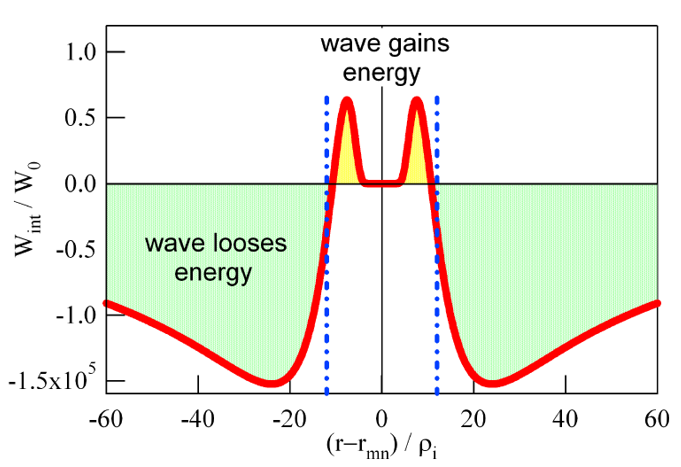
\includegraphics[width=0.70\textwidth]{Fig_Wint_resonance.png}
	\caption{Energy exchanged between a potential wave and the plasma particles as a function of the distance to a resonant surface}
	
	\label{fig:Wint_résonance}
\end{figure}
The most obvious result is that $W_{int}$ has well marked minima slightly beyond $x = x_T$ (values $x_T$ and $-x_T$ are indicated by vertical dashed lines). The negative values of $W_{int}$ at these positions indicate that the wave gives a large part of its energy away to the particlesz. The consequence of this loss is that the wave does not propagate beyond these minima. The interaction takes place in a region of width:
\[
		\Delta \simeq \frac{\omega}{\omega_T^*}\frac{L_s}{L_T}\rho_i
\]
around the so-called rational surfaces (i.e. characterised by a rational safety factor $q = m/n$). If the width $\Delta$ is smaller than the distance between rational surfaces $\Delta_r \simeq 1/k_{\theta s}$, the various modes are resonant in non-adjacent regions and thus cannot interact with each other. In the other case, they can transfer energy to each other through their exchanges with particles. On a macroscopic scale, this gives rise to transport. The boundary between these two regimes can be quantified with the Chirkov parameter:
\[
		\sigma_{Chir} = \frac{\Delta}{\Delta_r} = 1
\]
In a tokamak, we have in general $L_s \simeq 3$ m and $L_T \simeq 0,25$ m, and thus $\sigma_{Chir} > 1$. Tokamaks are in a regime where instabilities due to electrostatic potential fluctuations drive energy exchanges on the macrosopic scale. These exchanges are the expresion of turbulent transport.



		\section{Nature of turbulent modes: ITG, ETG and TEM}
		
As it was shown rapidly in the previous paragraph, the resonance condition refers to the fluctuation wavenumbers but also to a scale characteristic of the plasma particles. More specifically, if the characteristic scale of a particle type is large with respect to the wavelength of the considered mde, there is no interaction (no energy exchange): the particle population is adiabatic.

As a result, a categorisation of turbulent modes has been adopted. FThere are four classes of modes, related to the four types of plasma particles (passing and trapped electrons, passing and trapped ions, impurities being left aside since they are traces most of the time), of which the names are always referrred to in the turbulent transport studies.

They are the following, sorted by descending order of wavelength. The very large wavelength modes (larger than the ion banana width) are called TIM (\textit{Trapped Ion Modes}) because they interact with trapped ions. For wavelengths between the ion banana width and the ion Larmor radius, the modes are called ITG (\textit{Ion Temperature Gradient}) because they are destabilised when the ion temperature gradient is large (or equivalently when the gradient length is small compared with the plasma minor radius). For wavelengths between the ion Larmor radius and the electron banana width, the modes are called TEM (\textit{Trapped Electron Modes}). finally for wavelengths between the electron banana width and the electron Larmor radius, the modes are called ETG (\textit{Electron Temperature Gradient}).

In practice, the ion Larmor radius and the electron banana width are of the same order of magnitude. The ITG modes and  TEMs are thus present in the same wavelength range. The situation is sketched in Fig.  \ref{fig:_schéma_modes_turb}.
\begin{figure}[htbp]
	\centering
		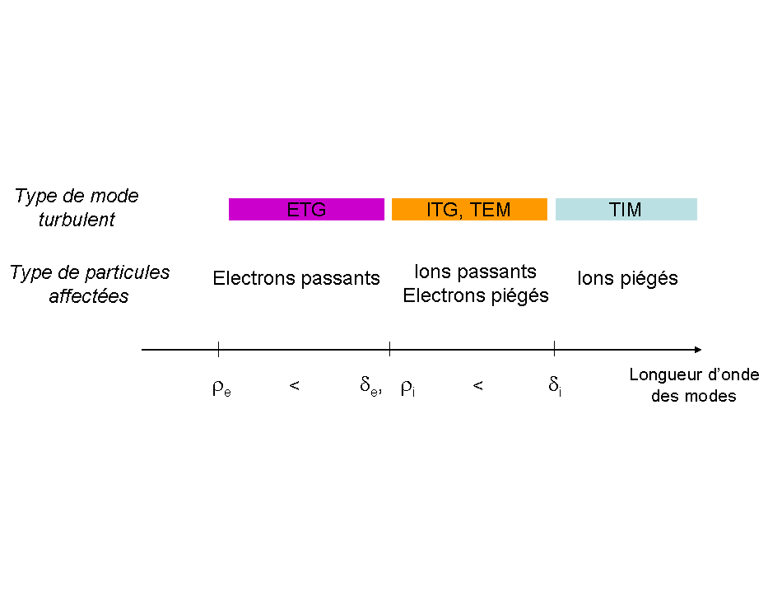
\includegraphics{Fig_schema_modes_turb.png}
	\caption{Turbulent mode classes a a function of wavelength. The type of particles interacting with the mode ins indicated.}
	\label{fig:_schéma_modes_turb}
\end{figure}

A detailed treatment shows that the ion type modes (ITG, TIM) rotate in the ion diamagnetic drift direction and the electron modes in the electron diamagnetic drift direction. It is one of the experimental tests which allwos to distinguish between ITG and TEM.

\textbf{NB 1:} The TIM modes, which could contribute to transport on a macroscopic scale, are never taken into account since their amplitude is weak.

\textbf{NB 2:} The ETG modes are small scale modes. Although always present, they contribute little to macroscopic transport. However, there are processes (not discussed in these notes) which allow these modes to transfer energy to longer wavelength modes. These processes coudl play an important role in improved confinement regimes, where large scale turbulence is strongly suppressed.





%		\section{Modèle du gradient critique}
		
		\section{Turbulent flux in the quasilinear theory}
		\label{FluxTurbulentsDansLaTheorieQuasiLineaire}

In order to determine the form of the turbulent particle and heat fluxes, we adopt the quasilinear gyrokinetic theory frame and we calculate the response $\tilde{f}$ of the distribution function to a perturbation $\tilde{H}$ of the hamiltonian. In general for $\tilde{H}$ an electrostatic potential perturbation is chosen. This a hypothesis of the model: we thus constrain the $k$ spectrum shape of turbulence as well as its amplitude. As a result, this model can be used to obtain the flux dependences on the plasma gradients but not their absolute values.

The fluxes take the well known form:
\[
	\Gamma_s = -D_s \nabla n_s + V_s n_s
\]
where the index $s$ stands for the particle type. The diffusion coefficient and the convection velocity are:
\begin{eqnarray*}
		D_s  &  =  &  \left( \frac{q}{rB} \right)^2 \sum_{n,\omega_0} n^2 \left< \sqrt{\frac{\xi}{\pi}} e^{-\xi}.\frac{\gamma_0}{\left( n\Omega_s(\xi,\lambda) - \omega_{r0} \right)^2 + \gamma_0^2} \right>_{\xi,\lambda} \left| \tilde{\phi}_n \right|^2		\\
		V_s  &  =  &  - C_s^{th} \frac{\nabla T_s}{T_s} + \frac{C_q^c}{R}
\end{eqnarray*}

The somewhat complicated expression of the diffusion coefficient does not allow to discuss easily the parameters on which it depends but the turbulent diffusion dependence on the squared modulus of the fluctuating potential is retrieved.

The convection velocity expression shows two terms. The first one,proportional to the normalised temperature gradient of the considered species is called thermodiffusion. The proportionality coefficient $C_s^{th}$ depends on $1/Z$ ($Z$ being the species charge). The electron thermodiffusive flux is thus in opposite direction of the ion and impurity flux. Calculations show that the direction of this thermodiffusive flux depends on the turbulence type. It is outward for electrons (inward for ions and impurities) when turbulence is of the electronic type and in the oppposite direction when turbulence is of the ion type.

The second term is called curvature term. It is the dominant term. The coefficient $C_q^c$ is porportional to the normalised $q$ gradient $\nabla q/q$. The resulting flux is directed inward if the magnetic shear $s$ is positive, and outward if $s$ is negative (the exact limit is not strictly 0 but a negative value between -1 and 0). An additional term is often included in the curvature term. It is called the parallel compressibility flux, which is small and in opposite direction with respect to the thermodiffusive flux.

%		\section{Tests expérimentaux}
		
%				\subsection{Mise en évidence des seuils}
				
%				\subsection{Rôle des gradients}
				
%				\subsection{Rôle de la charge des particules}
				
%				\subsection{Nature de la turbulence et renversement de convection}



% IV. Méthodes expérimentales (à écrire)
%\chapter{Méthodes expérimentales}

		\section{Méthode gradient-flux}

		\section{Résolution de l'équation de continuité}

		\section{Modulations et analyse de Fourier}
		
		\section{Transitoires et stationnaires (transport de la chaleur)}





%\bibliography{biblio_cours_transport_M2Fusion}
%%\bibliographystyle{plain}
%\bibliographystyle{these2}
%\pagebreak
%\strut\thispagestyle{empty}
%\vfill





%\backmatter

% \renewcommand{\chaptermark}[1]{\markboth{#1}{}}

%%\include{conclusion}

%\renewcommand{\footrulewidth}{0pt}

\pagestyle{plain}


%-----------------------------------------------------------------------------------


%%%%%%%%%%%%%%%%%%%%%%%%%%%%%%%%%%%%%%%%%%%%%%%%%%%%%%%%%%%%%%%%%%%%%%%%%%%%%%%
%                                BIBLIOGRAPHIE                                %
%%%%%%%%%%%%%%%%%%%%%%%%%%%%%%%%%%%%%%%%%%%%%%%%%%%%%%%%%%%%%%%%%%%%%%%%%%%%%%%


%\listoffigures
%\listoftables

\newpage

%\addcontentsline{toc}{part}{Références}
%\def\bibname{Références}

%\bibliographystyle{these2}
%\bibliography{biblio_these}
%\cleardoublepage
%\include{remerciements}

%\include{summary}

\end{document}
